\mychapter{\textsc{Resultados e Análises}}{chp:resultados}
\lhead{\textsc{Resultados e Análises}}

%Breve resumo do capítulo.
\lettrine{C}{om} a aplicação dos métodos explanados e a fundamentação teórica referendada, apresentamos os resultados, contextualizando com o problema central deste trabalho e objetivos propostos. 

Para a apresentação dos resultados subdividimos este capítulo em quatro partes, sendo as três primeiras referindo-se a cada uma das áreas pesquisadas, são elas: Características Estruturais das Redes, Medidas de Centralidade, Ranking das Medidas de Centralidade e Discussão dos Resultados.

Na primeira parte apresentamos os resultados das topologias das redes, número de vértices e arestas, características estruturais, densidades, coeficientes de clusterização. É apresentado também as matrizes de coautorias de cada área para todo o período por área.

Na segunda parte, são apresentadas os resultados das medidas de centralidade de cada rede: centralidade do grau (\textit{degree centrality}),  centralidade de proximidade (\textit{closeness centrality}), centralidade de intermediação (\textit{betweeness centrality}), com a apresentação dos gráficos comparativos entre o posicionamento da Universidade Federal de Alagoas (vértice focal), comparado de forma analítica em relação ao comportamento das medidas médias das Universidades Federais do Brasil, seguindo com as interpretações e análises dos resultados.

Na terceira parte, é apresentado o ranking dos índices aferidos por cada Unidade Federativa (UF) em cada área do conhecimento para cada medida de centralidade.

Na quarta parte, realizamos a discussão dos resultados; contextualizando os resultados das medidas de centralidade com a colaboração científica, entendendo o posicionamento do vértice focal (Alagoas) e o desempenho de cada UF em cada área.

\section{\textbf{Redes de Coutorias - Base SciELO}}

Neste ponto apresentamos a análise do comportamento e dos resultados das medidas de centralidade das redes de coautoria de artigos científicos indexados na base SciELO no período compreendido entre 2008 à 2017 para as áreas de: \textit{Health Sciences}, \textit{Agricultural Sciences}, \textit{Exact and Earth Sciences}.


\subsection{\textbf{Características Estruturais}}

Nesta seção trazemos a tona as características estruturais das redes objeto de estudo, sendo elas determinadas: Rede Brasil, compreendendo as Universidades Federais relacionadas ao respectivo Estado (UF - Unidade Federativa) às quais estão sediadas; para cada área do conhecimento visto acima.

Neste tópico apresentamos a estrutura da Rede Brasil com a finalidade de compreendermos a dimensão e topologia de cada área analisada dentro do período estudado. Na figura \ref{nos-arestas-todos}, verificamos o número de vértices e arestas para cada ano/área.


\begin{table}[H]
	\centering
	\begin{tabular}{lllllll}
		\hline
		\multicolumn{7}{|c|}{\textbf{Topologia: Vértices e Arestas por Área}}                                                                                                                                                                                                                                                                                                                                                                                            \\ \hline
		\rowcolor[HTML]{EFEFEF} 
		\multicolumn{1}{|l|}{\cellcolor[HTML]{EFEFEF}\textbf{Área}} & \multicolumn{2}{c|}{\cellcolor[HTML]{EFEFEF}\textbf{\begin{tabular}[c]{@{}c@{}}Health \\ Sciences\end{tabular}}}               & \multicolumn{2}{c|}{\cellcolor[HTML]{EFEFEF}\textbf{\begin{tabular}[c]{@{}c@{}}Agricultural \\ Sciences\end{tabular}}}         & \multicolumn{2}{c|}{\cellcolor[HTML]{EFEFEF}\textbf{\begin{tabular}[c]{@{}c@{}}Exact and Earth \\ Sciences\end{tabular}}}      \\ \hline
		\rowcolor[HTML]{C0C0C0} 
		\multicolumn{1}{|l|}{\cellcolor[HTML]{C0C0C0}\textbf{Ano}}  & \multicolumn{1}{l|}{\cellcolor[HTML]{C0C0C0}\textbf{Vértices}} & \multicolumn{1}{l|}{\cellcolor[HTML]{C0C0C0}\textbf{Arestas}} & \multicolumn{1}{l|}{\cellcolor[HTML]{C0C0C0}\textbf{Vértices}} & \multicolumn{1}{l|}{\cellcolor[HTML]{C0C0C0}\textbf{Arestas}} & \multicolumn{1}{l|}{\cellcolor[HTML]{C0C0C0}\textbf{Vértices}} & \multicolumn{1}{l|}{\cellcolor[HTML]{C0C0C0}\textbf{Arestas}} \\ \hline
		\multicolumn{1}{|l|}{2008}                                  & \multicolumn{1}{l|}{27}                                        & \multicolumn{1}{l|}{109}                                      & \multicolumn{1}{l|}{25}                                        & \multicolumn{1}{l|}{90}                                       & \multicolumn{1}{l|}{21}                                        & \multicolumn{1}{l|}{63}                                       \\ \hline
		\multicolumn{1}{|l|}{2009}                                  & \multicolumn{1}{l|}{25}                                        & \multicolumn{1}{l|}{122}                                      & \multicolumn{1}{l|}{26}                                        & \multicolumn{1}{l|}{100}                                      & \multicolumn{1}{l|}{25}                                        & \multicolumn{1}{l|}{87}                                       \\ \hline
		\multicolumn{1}{|l|}{2010}                                  & \multicolumn{1}{l|}{25}                                        & \multicolumn{1}{l|}{163}                                      & \multicolumn{1}{l|}{25}                                        & \multicolumn{1}{l|}{154}                                      & \multicolumn{1}{l|}{22}                                        & \multicolumn{1}{l|}{91}                                       \\ \hline
		\multicolumn{1}{|l|}{2011}                                  & \multicolumn{1}{l|}{25}                                        & \multicolumn{1}{l|}{165}                                      & \multicolumn{1}{l|}{27}                                        & \multicolumn{1}{l|}{150}                                      & \multicolumn{1}{l|}{23}                                        & \multicolumn{1}{l|}{88}                                       \\ \hline
		\multicolumn{1}{|l|}{2012}                                  & \multicolumn{1}{l|}{26}                                        & \multicolumn{1}{l|}{181}                                      & \multicolumn{1}{l|}{26}                                        & \multicolumn{1}{l|}{180}                                      & \multicolumn{1}{l|}{24}                                        & \multicolumn{1}{l|}{88}                                       \\ \hline
		\multicolumn{1}{|l|}{2013}                                  & \multicolumn{1}{l|}{26}                                        & \multicolumn{1}{l|}{183}                                      & \multicolumn{1}{l|}{26}                                        & \multicolumn{1}{l|}{178}                                      & \multicolumn{1}{l|}{22}                                        & \multicolumn{1}{l|}{86}                                       \\ \hline
		\multicolumn{1}{|l|}{2014}                                  & \multicolumn{1}{l|}{26}                                        & \multicolumn{1}{l|}{197}                                      & \multicolumn{1}{l|}{27}                                        & \multicolumn{1}{l|}{179}                                      & \multicolumn{1}{l|}{25}                                        & \multicolumn{1}{l|}{83}                                       \\ \hline
		\multicolumn{1}{|l|}{2015}                                  & \multicolumn{1}{l|}{27}                                        & \multicolumn{1}{l|}{194}                                      & \multicolumn{1}{l|}{26}                                        & \multicolumn{1}{l|}{173}                                      & \multicolumn{1}{l|}{22}                                        & \multicolumn{1}{l|}{77}                                       \\ \hline
		\multicolumn{1}{|l|}{2016}                                  & \multicolumn{1}{l|}{26}                                        & \multicolumn{1}{l|}{298}                                      & \multicolumn{1}{l|}{26}                                        & \multicolumn{1}{l|}{182}                                      & \multicolumn{1}{l|}{25}                                        & \multicolumn{1}{l|}{99}                                       \\ \hline
		\multicolumn{1}{|l|}{2017}                                  & \multicolumn{1}{l|}{26}                                        & \multicolumn{1}{l|}{199}                                      & \multicolumn{1}{l|}{25}                                        & \multicolumn{1}{l|}{190}                                      & \multicolumn{1}{l|}{24}                                        & \multicolumn{1}{l|}{94}                                       \\ \hline
	\end{tabular}
\label{nos-arestas-todos}
\caption{Topologia das Redes (Vértices e Arestas) por Ano}
\end{table}


Pela topologia verificamos que as área de \textit{Health Sciences} e \textit{Agricultural Sciences} possuem um maior número de arestas ao logo do tempo quando comparada a \textit{Exact and Earth Sciences}. Destaque para o ano de 2016 em que observamos um pico que eleva o número de arestas no ano de 2016, como visto na tabela \ref{nos-arestas-todos} o que possivelmente neste ano maior número de publicações/indexações foram realizadas, o que resultou o aumento da conectividade da rede, que impactou em sua densidade e também no resultados das medidas de centralidade como veremos a frente. 

Em \textit{Agricultural Sciences} podemos considerar uma normalidade, considerando o número médio de vértices e uma tendência crescente de arestas (coautorias) ao longo do tempo; \textit{Exact and Earth Sciences} possui uma observação curiosa pela oscilação do número de vértices de cada ano, ou seja a desconexão e reconexão destes, mostrando que ao longo do tempo as participações do estados nas coautorias, em outros anos alguns estados deixaram de colaborar e participar da rede.

A tabela \ref{estruturais} abaixo apresenta a densidade e aglomeração (clustering coefficient) para complementar a compreensão da estrutura e dimensão de cada rede, que caracteriza as relações de coautorias existentes em cada área.

\begin{table}[H]
	\centering
	\begin{tabular}{|l|l|l|l|l|l|l|}
		\hline
		\multicolumn{7}{|c|}{\textbf{Características Estruturais da Rede Brasil por Área}}                                                                                                                                                                                                                                                                                                                                 \\ \hline
		\rowcolor[HTML]{C0C0C0} 
		\multicolumn{4}{|c|}{\cellcolor[HTML]{C0C0C0}\textbf{Densidade}}                                                                                                                                           & \multicolumn{3}{c|}{\cellcolor[HTML]{C0C0C0}\textbf{Aglomeração (Clustering Coefficient)}}                                                                                                          \\ \hline
		\rowcolor[HTML]{EFEFEF} 
		Ano  & \begin{tabular}[c]{@{}l@{}}Health \\ Sciences\end{tabular} & \begin{tabular}[c]{@{}l@{}}Agricultural \\ Sciences\end{tabular} & \begin{tabular}[c]{@{}l@{}}Exact and Earth \\ Sciences\end{tabular} & \begin{tabular}[c]{@{}l@{}}Health \\ Sciences\end{tabular} & \begin{tabular}[c]{@{}l@{}}Agricultural \\ Sciences\end{tabular} & \begin{tabular}[c]{@{}l@{}}Exact and Earth \\ Sciences\end{tabular} \\ \hline
		2008 & 0,121                                                      & 0,155                                                            & 0,150                                                                & 0,523                                                      & 0,364                                                            & 0,355                                                               \\ \hline
		2009 & 0,165                                                      & 0,152                                                            & 0,145                                                               & 0,625                                                      & 0,415                                                            & 0,398                                                               \\ \hline
		2010 & 0,230                                                       & 0,258                                                            & 0,197                                                               & 0,726                                                      & 0,557                                                            & 0,506                                                               \\ \hline
		2011 & 0,235                                                      & 0,214                                                            & 0,174                                                               & 0,744                                                      & 0,543                                                            & 0,356                                                               \\ \hline
		2012 & 0,238                                                      & 0,271                                                            & 0,159                                                               & 0,773                                                      & 0,601                                                            & 0,391                                                               \\ \hline
		2013 & 0,242                                                      & 0,271                                                            & 0,186                                                               & 0,772                                                      & 0,619                                                            & 0,429                                                               \\ \hline
		2014 & 0,265                                                      & 0,252                                                            & 0,138                                                               & 0,745                                                      & 0,619                                                            & 0,395                                                               \\ \hline
		2015 & 0,238                                                      & 0,258                                                            & 0,167                                                               & 0,803                                                      & 0,608                                                            & 0,339                                                               \\ \hline
		2016 & 0,418                                                      & 0,282                                                            & 0,165                                                               & 0,943                                                      & 0,642                                                            & 0,489                                                               \\ \hline
		2017 & 0,266                                                      & 0,313                                                            & 0,170                                                                & 0,798                                                      & 0,682                                                            & 0,422                                                               \\ \hline
	\end{tabular}
\caption{Características Estruturais Rede Brasil (2008-2017)}
\label{estruturais}
\end{table}


\subsubsection{\textbf{Matrizes de Coautorias por Unidades Federativas}}

A seguir apresentamos as matrizes de coautorias por Unidades Federativas por área, compreendendo todo o período (2008 à 2017). As matrizes é uma das formas primárias de observar a colaboração científica existente entre os estados, e nos referenciaremos a elas, ao longo das análises dos resultados das medidas de centralidade.

\subsubsection{Health Sciences}

\begin{figure}[H]
	\begin{adjustwidth}{-.6in}{-.6in}
		\centering
		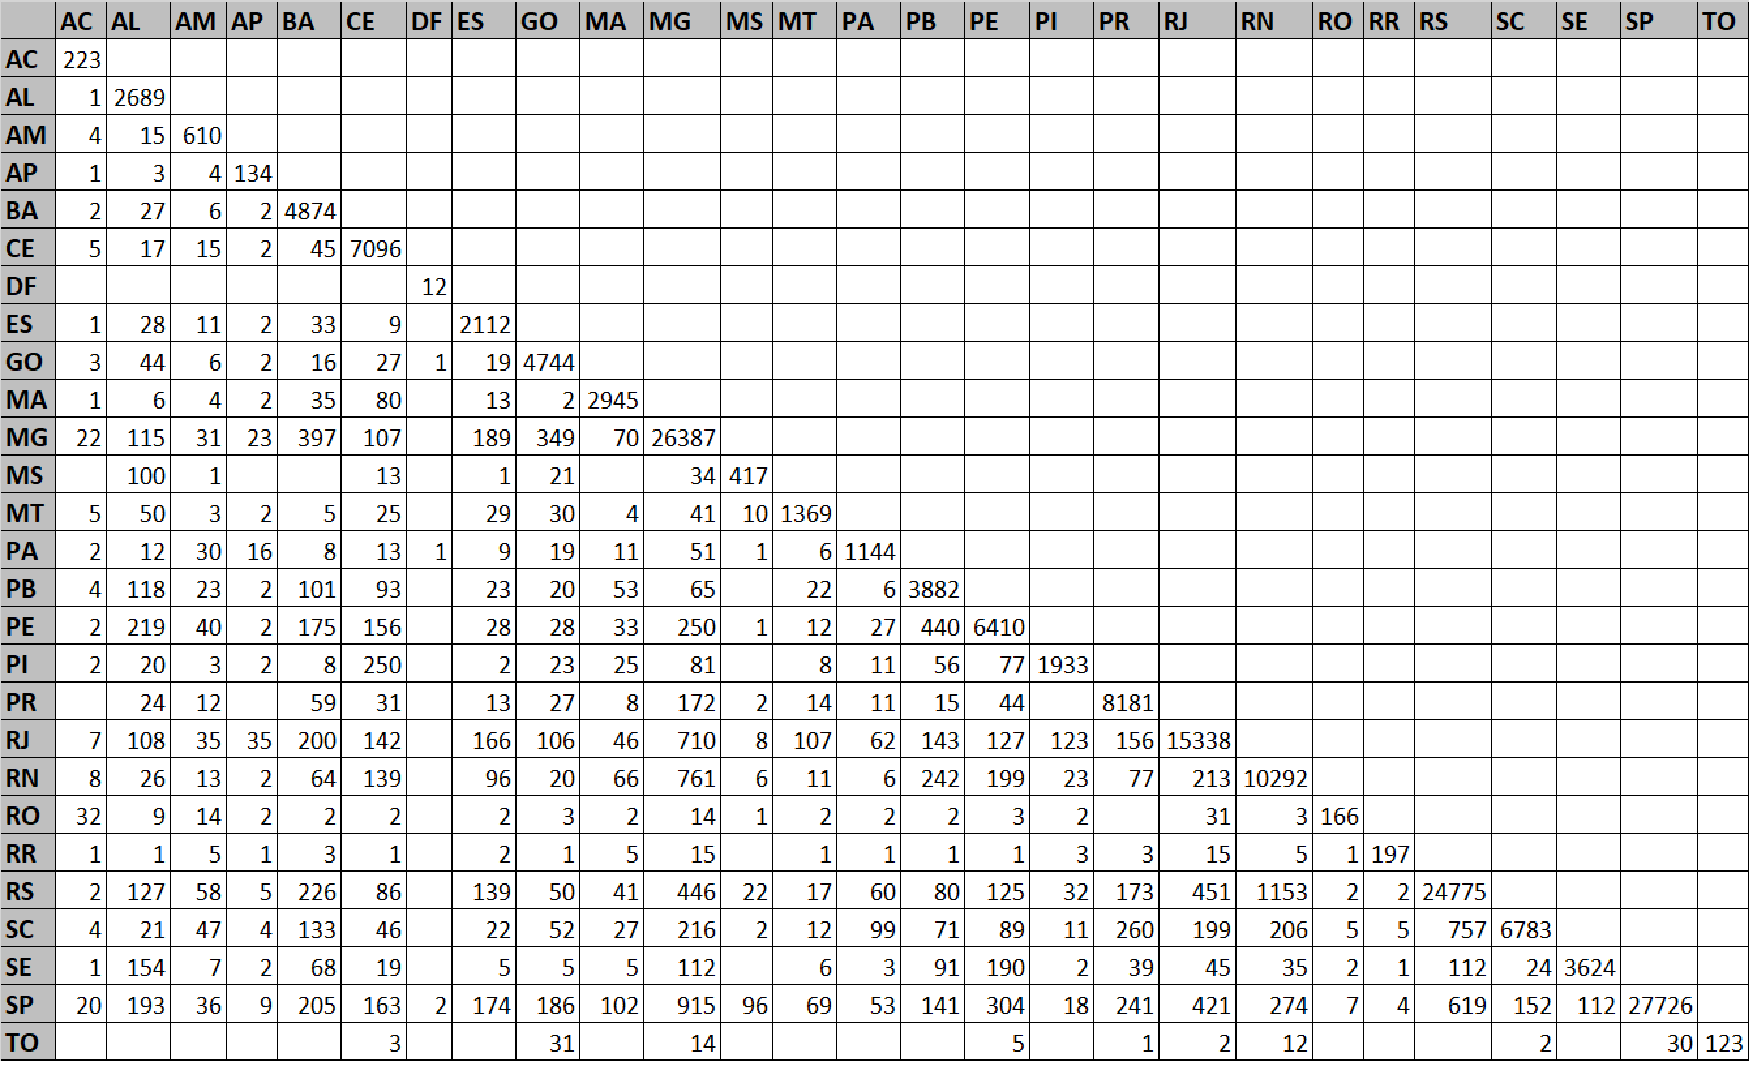
\includegraphics[scale=0.6]{Imagens/health/matriz-uf.pdf}
		\caption{Matriz de Coautorias \textit{Health Sciences} (2008-2017)}
		\label{matriz-uf-agri}
	\end{adjustwidth}
\end{figure}

Observamos para todo período analisado que a matriz na área de \textit{Health Sciences}, os valores absolutos de coautorias entre os estado, denota uma forte conectividade desta rede, quando comparada as áreas de \textit{Agricultural Sciences e Exact and Earth Sciences}, exceto para alguns estados, da região Norte do país, como Tocantins e Roraima. Podemos perceber o grande volume de coautorias existente dentro do mesmo estado, como São Paulo, Rio Grande do Sul, Minas Gerais e Rio de Janeiro.

\subsubsection{Agricultural Sciences}

\begin{figure}[H]
	\begin{adjustwidth}{-.6in}{-.6in}
		\centering
		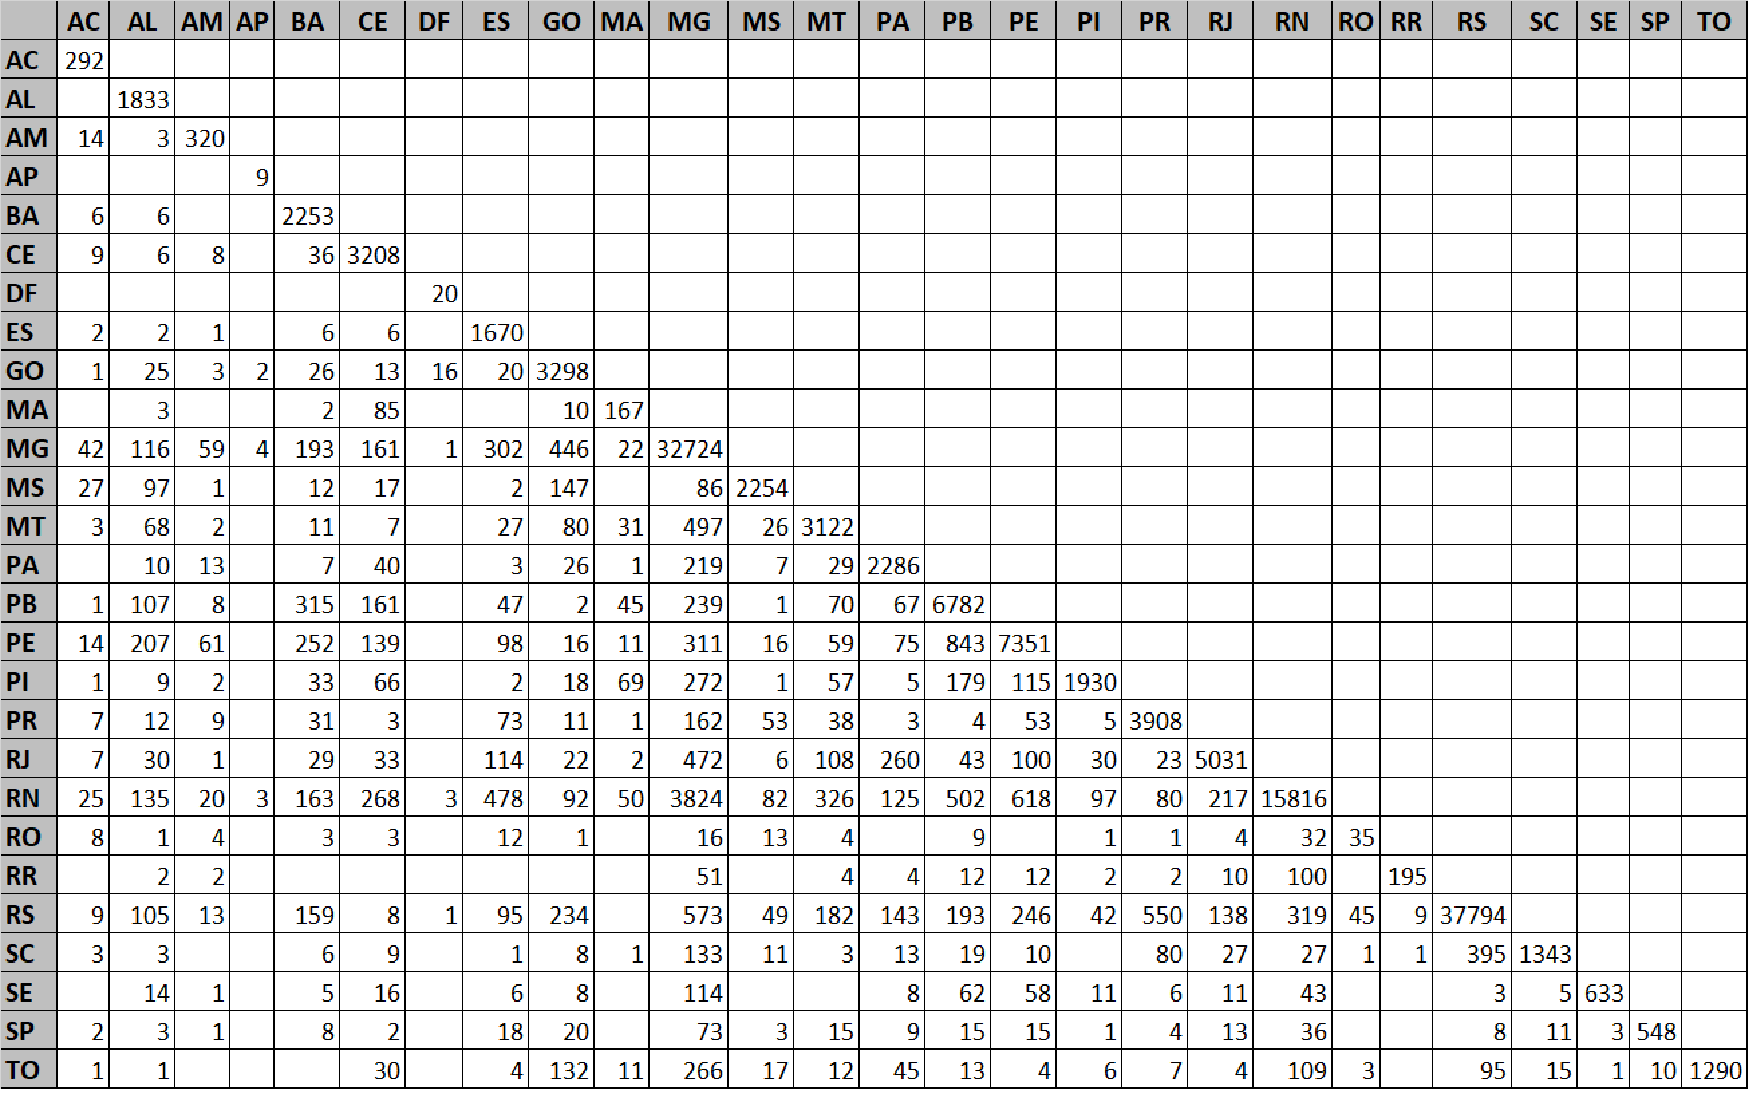
\includegraphics[scale=0.6]{Imagens/agricultural/matriz-uf.pdf}
		\caption{Matriz de Coautorias \textit{Agricultural Sciences} (2008-2017)}
		\label{matriz-uf-agri}
	\end{adjustwidth}
\end{figure}

Com a matriz de coautorias na área de \textit{Agricultural Sciences}, percebemos uma densidade menor e muitas lacunas da colaboração entre alguns unidades federativas, como o Distrito Federal, Roraima, e pouca volume em número de coautorias entre diversos estados. Destaque para o estado do Rio Grande do Sul, e no nordeste o Rio Grande do Norte, que por meio de suas  Universidade Federal do Rio Grande do Norte e da Universidade Federal Rural do Semi-Árido, apresentaram grande participação nas coautorias em Ciências Agrárias.

\subsubsection{Exact and Earth Sciences}

\begin{figure}[H]
	\begin{adjustwidth}{-.6in}{-.6in}
		\centering
		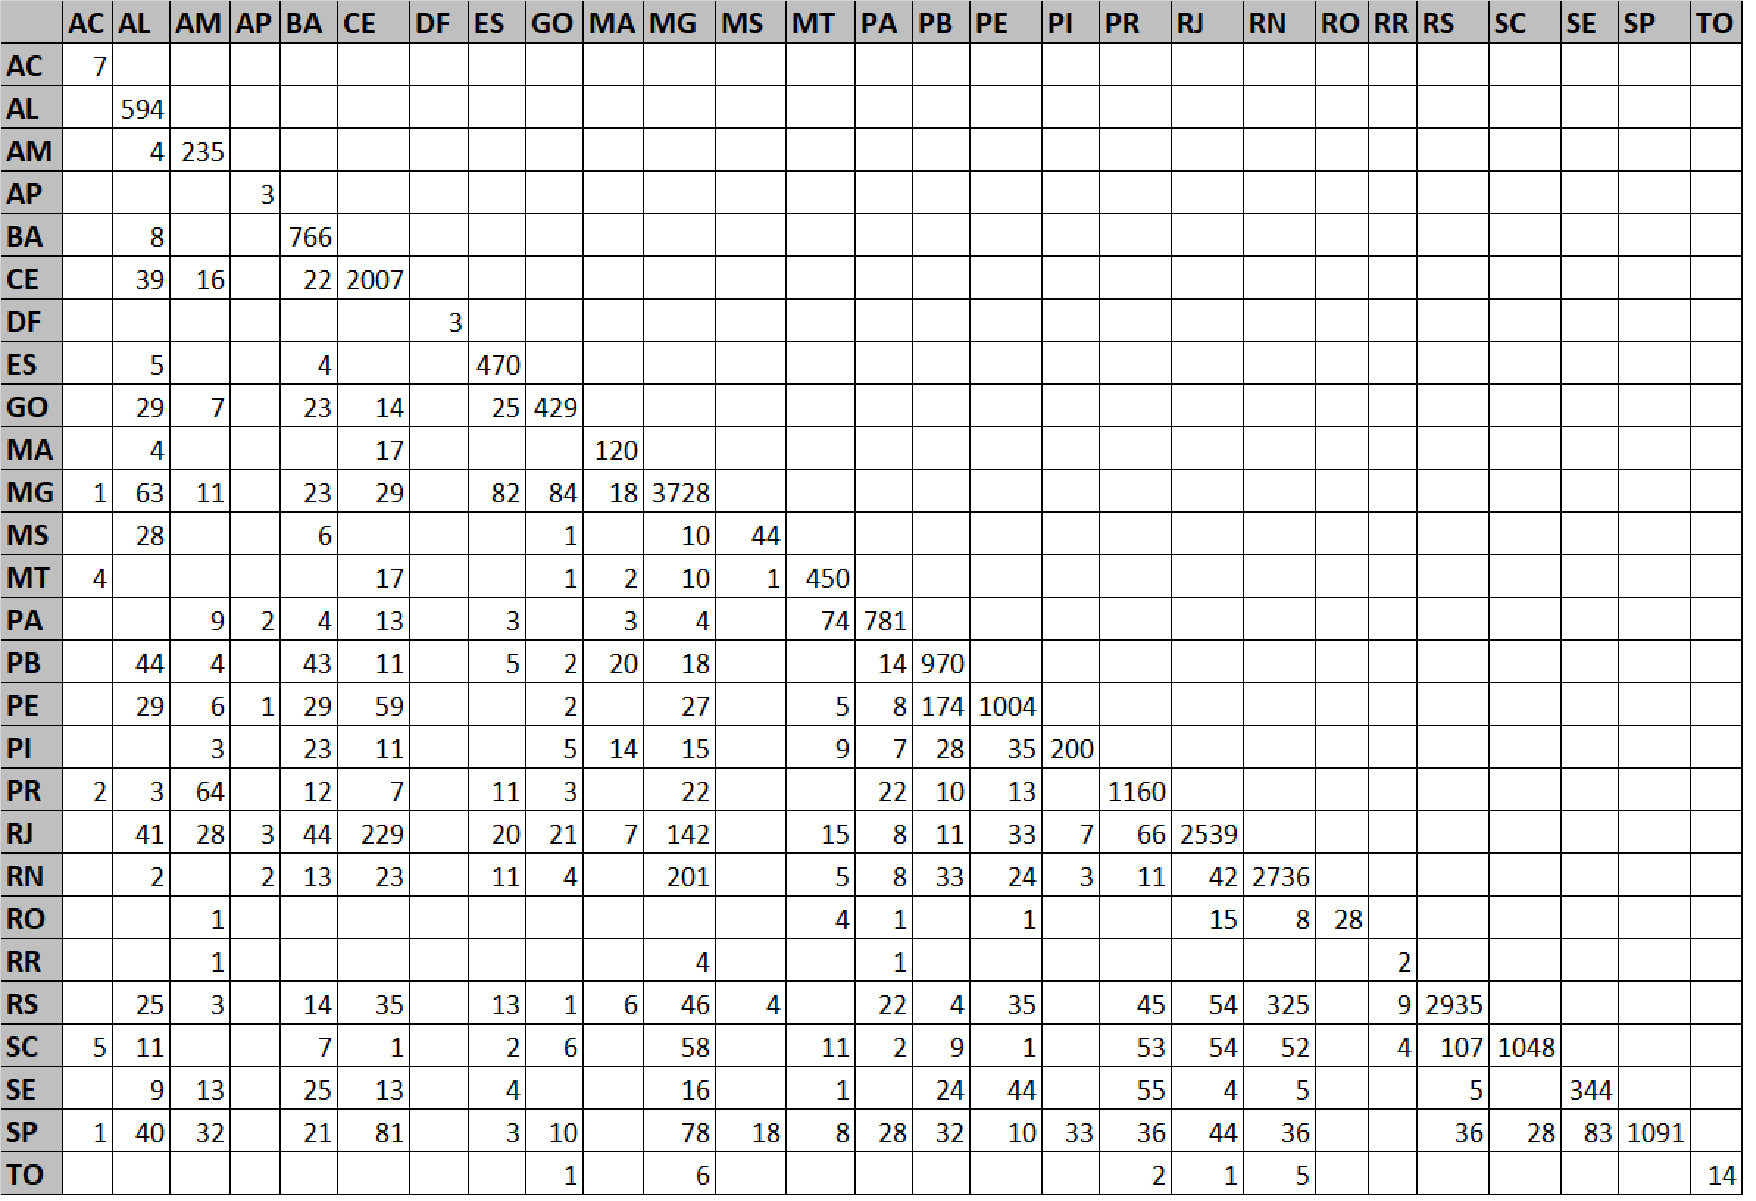
\includegraphics[scale=0.6]{Imagens/exact/matriz-uf.pdf}
		\caption{Matriz de Coautorias \textit{Exact and Earth Sciences} (2008-2017)}
		\label{matriz-agri}
	\end{adjustwidth}
\end{figure}

Em \textit{Exact and Earth Sciences} percebemos que pelo volume de coautoria, a Base SciELO não é um referência para a indexação de artigos nesta área, sua matriz apresenta poucas coautorias, realizada entre alguns estados, apresentando muitas lacunas principalmente em estados do Centro-Oeste e Norte do país. Destaque para Minas Gerais e Rio de Janeiro.

\subsubsection{Visualização da rede}

Para inspeção visual que coaduna com as análises numéricas, postamos a seguir, por seleção aleatória o ano de 2015 a rede de \textit{Agricultural Sciences} para Rede Brasil e Rede Alagoas, trata-se de uma plotagem exemplo uma vez que estamos trabalhando com 60 redes ao total, todas as redes (de cada ano e área) estão disponíveis no Apêndice \ref{redes}.


\begin{figure}[H]
\centering
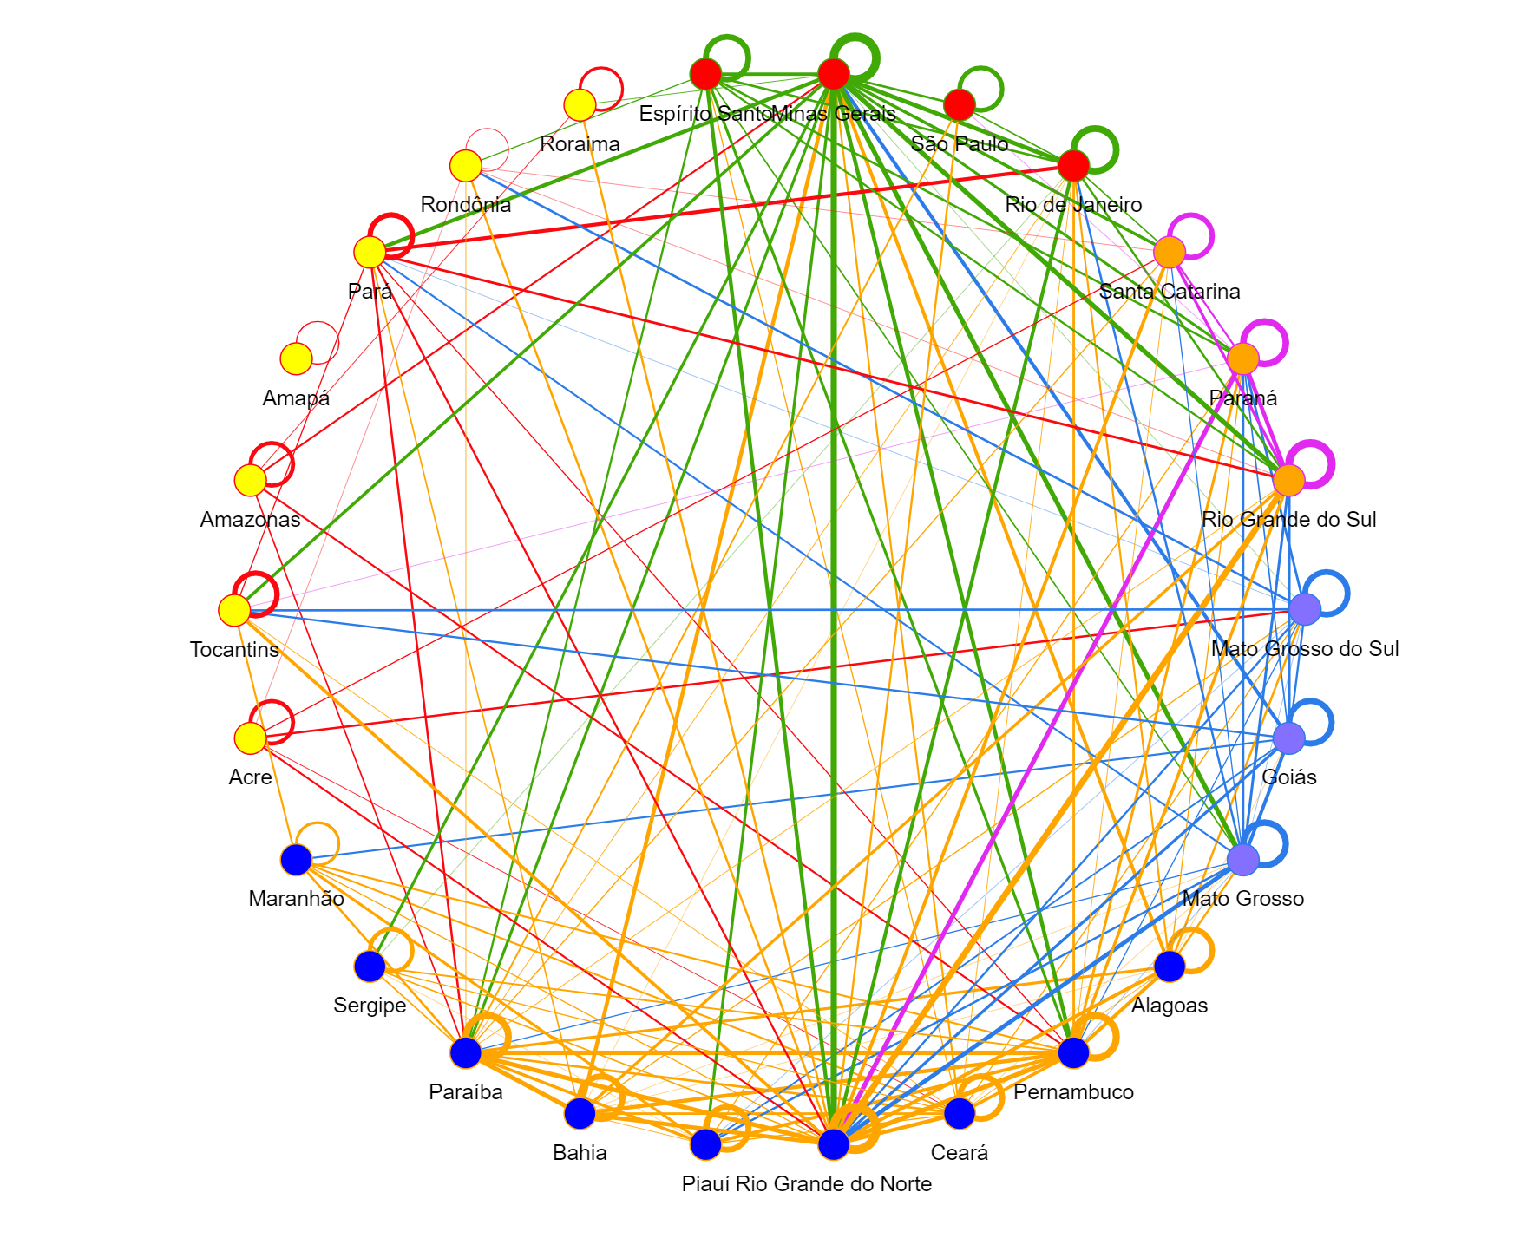
\includegraphics[scale=0.6]{Imagens/rede-agr-br-2015.pdf}
\caption{Rede de Coautoria das Universidades Federais do Brasil - 2015 (\textit{Agricultural Sciences})}
\label{rede-2015-br}
\end{figure}

As características propostas na plotagem da rede é, formato em círculo para fins comparativos, disposição dos vértices com coloração das UF pertencentes a mesma região geográfica, espessura e coloração das arestas indicando o maior volume/peso das coautorias existente entre as UFs, espessuras dos laços, indicando peso das coautorias existentes na mesma UF.

A figura \ref{rede-2015-br} apresenta a rede de coautoria das Universidades Federais do Brasil, composta pelos vértices que representam os Estados (Unidades Federativas - UF) do Brasil e suas ligações (arestas) representando as coautorias existentes entre eles. A figura \ref{rede-2015-al} representa para o mesmo ano e área a rede plotada a partir do vértice Alagoas.

\begin{figure}[H]
	\centering
	\includegraphics[scale=0.6]{Imagens/rede-agr-al-2015.pdf}
	\caption{Rede de Coautoria Vértice Focal Universidade Federal de Alagoas - 2015 (\textit{Agricultural Sciences})}
	\label{rede-2015-al}
\end{figure}

\section{\textbf{Medidas de Centralidade}}

Nesta seção, após a análise das características estruturais das Redes Brasil para cada área do conhecimento, determinamos o vértice focal de Alagoas, como Rede Alagoas, representado pela Universidade Federal de Alagoas, como ponto de interesse para uma avaliação do posicionamento e desempenho desta rede/vértice em comparação a Rede Brasil (média). Sendo esta, organizada por subseções para cada medida de centralidade.

Após a análise de cada medida, será apresentado um Ranking por cada área do e o o respectivo índice médio do período (2008-2017) para cada Unidade Federativa (UF). 

Válido ressaltar que foge ao escopo desse trabalho o entendimento de fatores exógenos ou específicos que não seja o do estudo das medidas de centralidade aplicadas a avaliação da colaboração científica, considerando que há várias possibilidades de investigações \textit{drill-down} que possam detalhar conhecimento complementares a respeito das coautorias. Os gráficos estão plotados em resolução maior no Apêndice \ref{graficos}.

\subsection{\textbf{Centralidade do Grau}}

Esta medida indica o melhor posicionamento dos vértices utilizando o parâmetro que possuem o maior número de ligações entre outros vértices, ou seja, a partir desse ponto de vista são vértices mais influentes, observaremos graficamente como se comportou a Rede Alagoas face a média da Rede Brasil.

A tabela \ref{degree-tab} apresenta os resultados da centralidade do grau para todas áreas comparando a Rede Brasil (média) e Alagoas.

\begin{table}[H]
	\centering
	\begin{tabular}{|l|l|l|l|l|l|l|}
		\hline
		\multicolumn{7}{|c|}{\textbf{\begin{tabular}[c]{@{}c@{}}Centralidade do Grau  \\ (Degree centrality) por Área\end{tabular}}}                                                                                                                                                                                                                                                          \\ \hline
		\rowcolor[HTML]{C0C0C0} 
		\textbf{Ano}  & \multicolumn{2}{c|}{\cellcolor[HTML]{C0C0C0}\textbf{\begin{tabular}[c]{@{}c@{}}Health \\ Sciences\end{tabular}}} & \multicolumn{2}{c|}{\cellcolor[HTML]{C0C0C0}\textbf{\begin{tabular}[c]{@{}c@{}}Agricultural \\ Sciences\end{tabular}}} & \multicolumn{2}{|c|}{\cellcolor[HTML]{C0C0C0}\textbf{\begin{tabular}[c]{@{}c@{}}Exact and \\ Earth Sciences\end{tabular}}} \\ \hline
		\rowcolor[HTML]{EFEFEF} 
		\textbf{Rede} & \textbf{Brasil}                                        & \textbf{Alagoas}                                        & \textbf{Brasil}                                           & \textbf{Alagoas}                                           & \textbf{Brasil}                                             & \textbf{Alagoas}                                            \\ \hline
		2008          & 6,29                                                   & 7                                                       & 7,44                                                      & 5                                                          & 8,19                                                        & 2                                                           \\ \hline
		2009          & 7,92                                                   & 7                                                       & 7,62                                                      & 8                                                         & 10,24                                                       & 14                                                          \\ \hline
		2010          & 11,04                                                  & 15                                                      & 12,40                                                     & 12                                                         & 12,55                                                       & 14                                                          \\ \hline
		2011          & 11,28                                                  & 10                                                      & 11,11                                                     & 13                                                         & 11,30                                                       & 12                                                          \\ \hline
		2012          & 11,92                                                  & 12                                                      & 13,54                                                     & 15                                                         & 10,67                                                       & 18                                                          \\ \hline
		2013          & 12,07                                                  & 14                                                      & 13,54                                                     & 14                                                         & 12,00                                                       & 12                                                          \\ \hline
		2014          & 13,23                                                  & 18                                                      & 13,11                                                     & 13                                                         & 9,44                                                        & 14                                                          \\ \hline
		2015          & 12,37                                                  & 19                                                      & 12,92                                                     & 13                                                         & 10,36                                                       & 6                                                           \\ \hline
		2016          & 20,92                                                  & 24                                                      & 14,08                                                     & 12                                                         & 12,32                                                       & 12                                                          \\ \hline
		2017          & 13,30                                                  & 19                                                      & 15,04                                                     & 15                                                         & 12,17                                                       & 14                                                          \\ \hline
	\end{tabular}
	\caption{Medidas de Centralidade do Grau por Área (2008-2017)}
	\label{degree-tab}
\end{table}

\subsubsection{Health Sciences}

\begin{figure}[H]
\centering
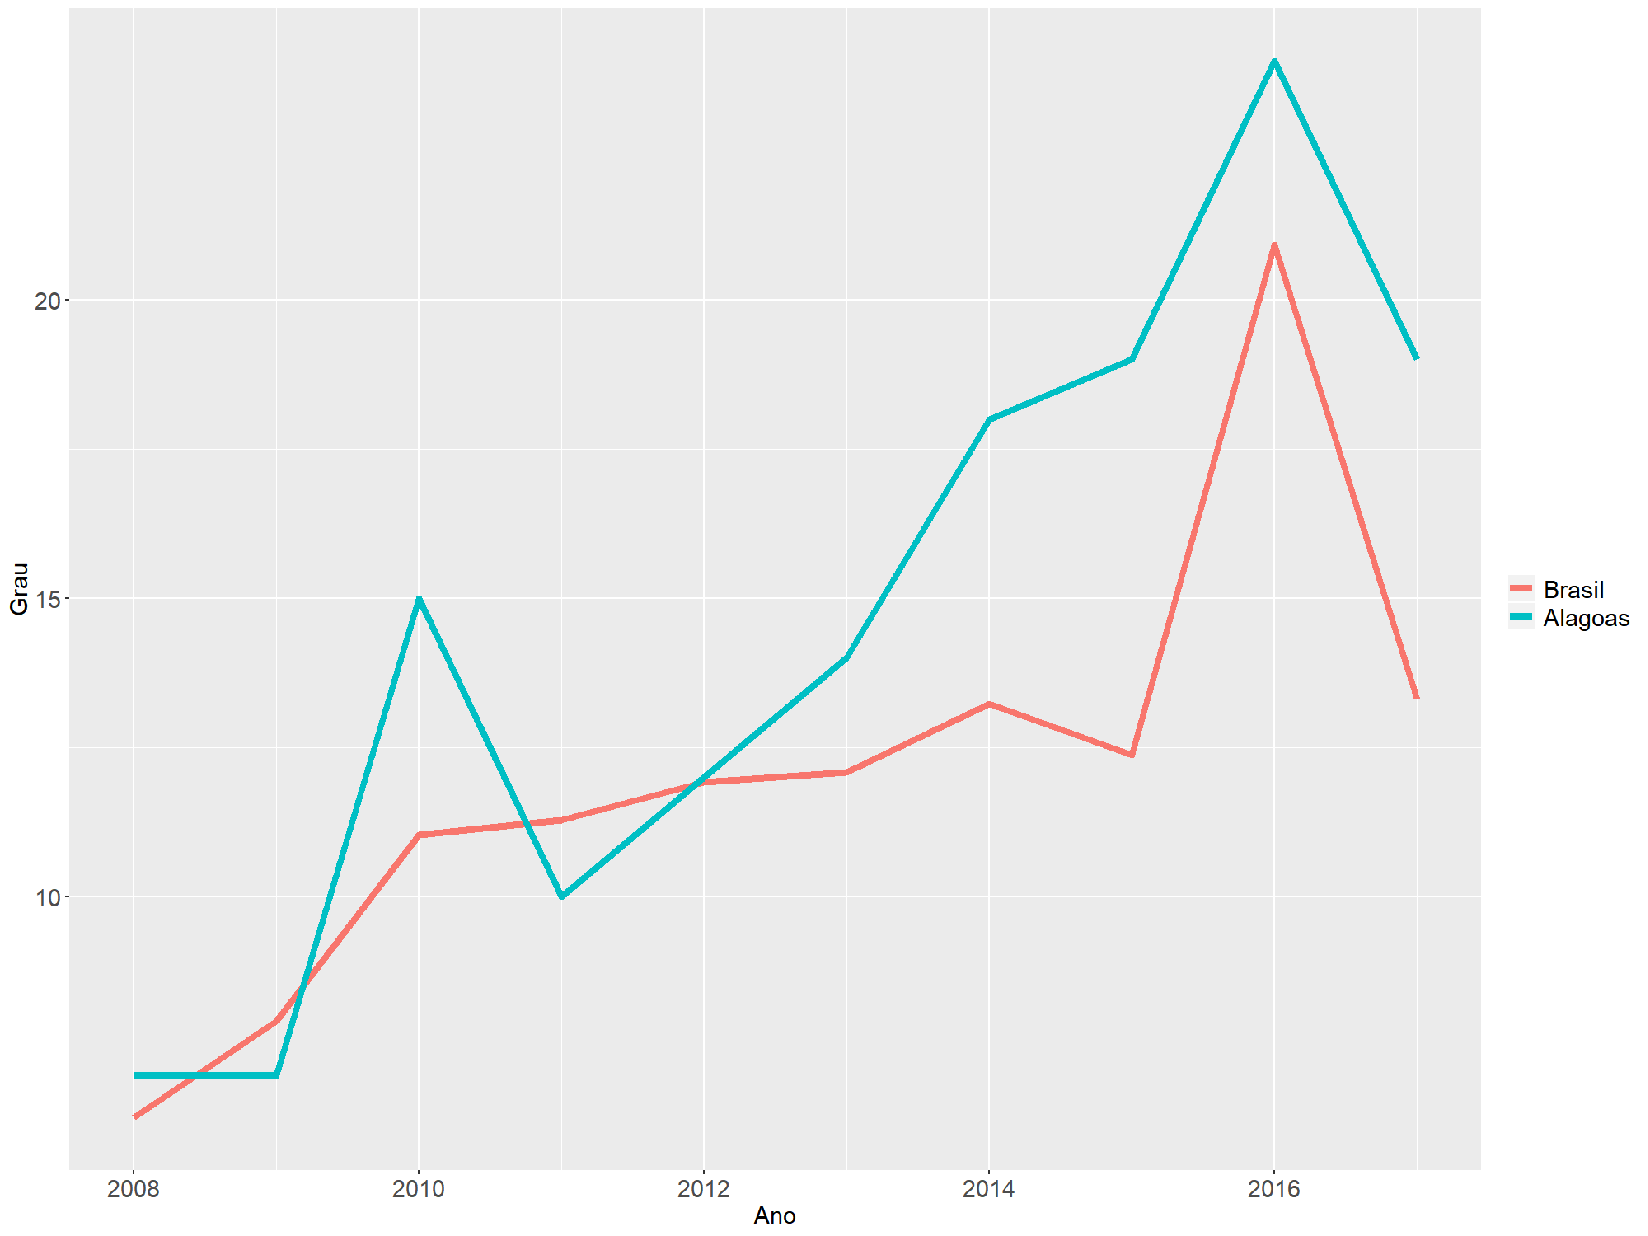
\includegraphics[scale=0.4]{Imagens/graf-linha-degree-br-al.pdf}
\caption{Centralidade do Grau (\textit{Health Sciences})}
\label{degree-health-1}
\end{figure}

\subsubsection{Agricultural Sciences}

\begin{figure}[H]
	\centering
	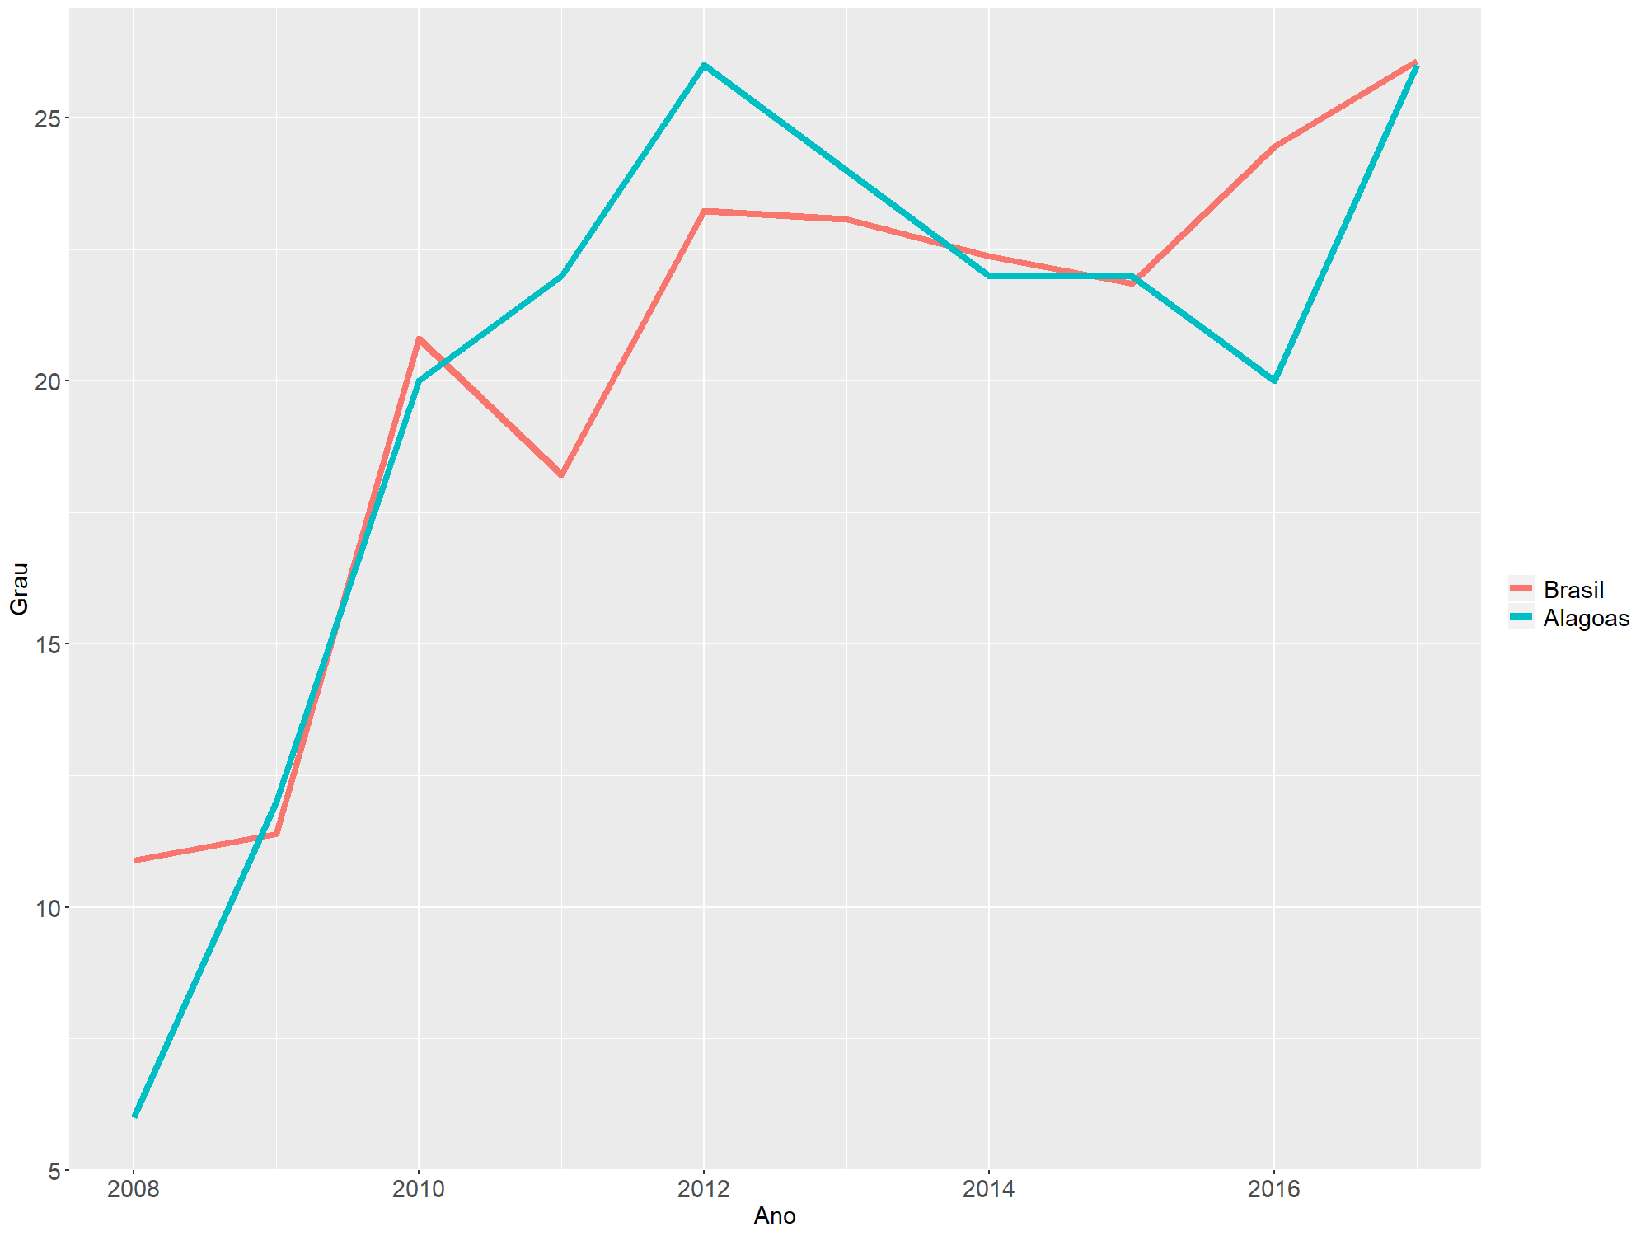
\includegraphics[scale=0.4]{Imagens/agricultural/graf-linha-degree-br-al.pdf}
	\caption{Centralidade do Grau (\textit{Agricultural Sciences})}
	\label{degree-agri-1}
\end{figure}

\subsubsection{Exact and Earth Sciences}

\begin{figure}[H]
	\centering
	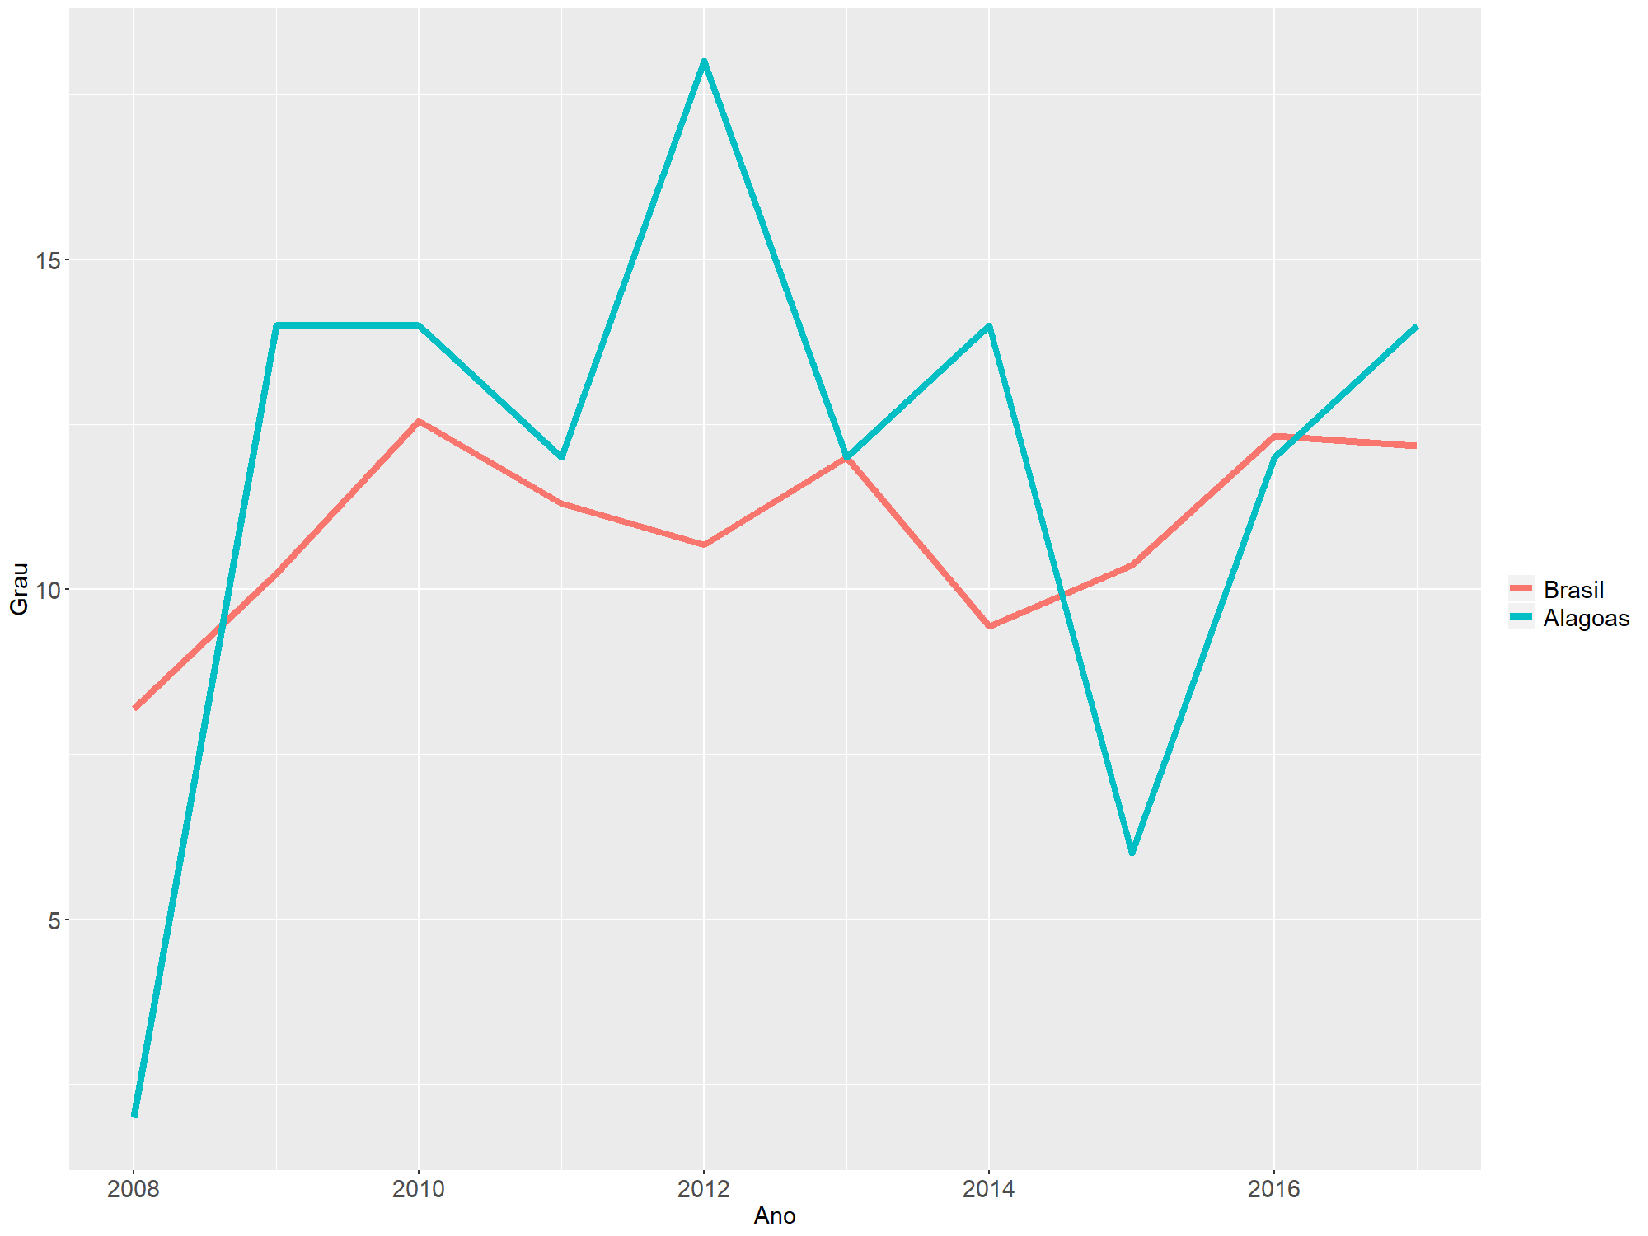
\includegraphics[scale=0.4]{Imagens/exact/graf-linha-degree-br-al.pdf}
	\caption{Centralidade do Grau (\textit{Exact and Earth Sciences})}
	\label{degree-exact-1}
\end{figure}

Os gráficos \ref{degree-health-1}, \ref{degree-agri-1} e \ref{degree-exact-1}, apresentam respectivamente as curvas na série temporal (2008-2017) da centralidade do grau da média da Rede Brasil e Alagoas. 

Na disposição das curvas na área de \textit{Health Sciences}, sendo Rede Brasil (vermelha) e Alagoas (azul), percebemos ao longo do período projeção em direção análoga, e que exceto como aferido no ano de 2009 e 2011, Alagoas esteve com a centralidade do grau maior que a média do Brasil. O que nos levar a inferir que nesse período

O gráfico \ref{degree-agri-1} mostra que Alagoas andou muito próximo da média do Brasil para \textit{Agricultural Sciences} para este indicador. Destaque para o ano de 2012, em que obteve o maior índice de centralidade na rede, estas razões podem ser investigadas com maior detalhamento sobre as ocorrências das coautorias neste ano.

A análise da centralidae para área de \textit{Exact and Earth Sciences} mostra que apesar de não ser uma área de grande volume de artigos indexados na base SciELO, a partir de 2009, Alagoas obteve um índice de centralidade maior que a média da rede. Com um queda considerável do seu índice em 2015, como dito uma análise investigatória poderá responder o que ocorreu neste ano, como a desconexão com outros vértices, não ocorrendo coautorias em pares com outros estados.

%% HISTOGRAMAS GRAU

\begin{figure}[H]
	\centering
	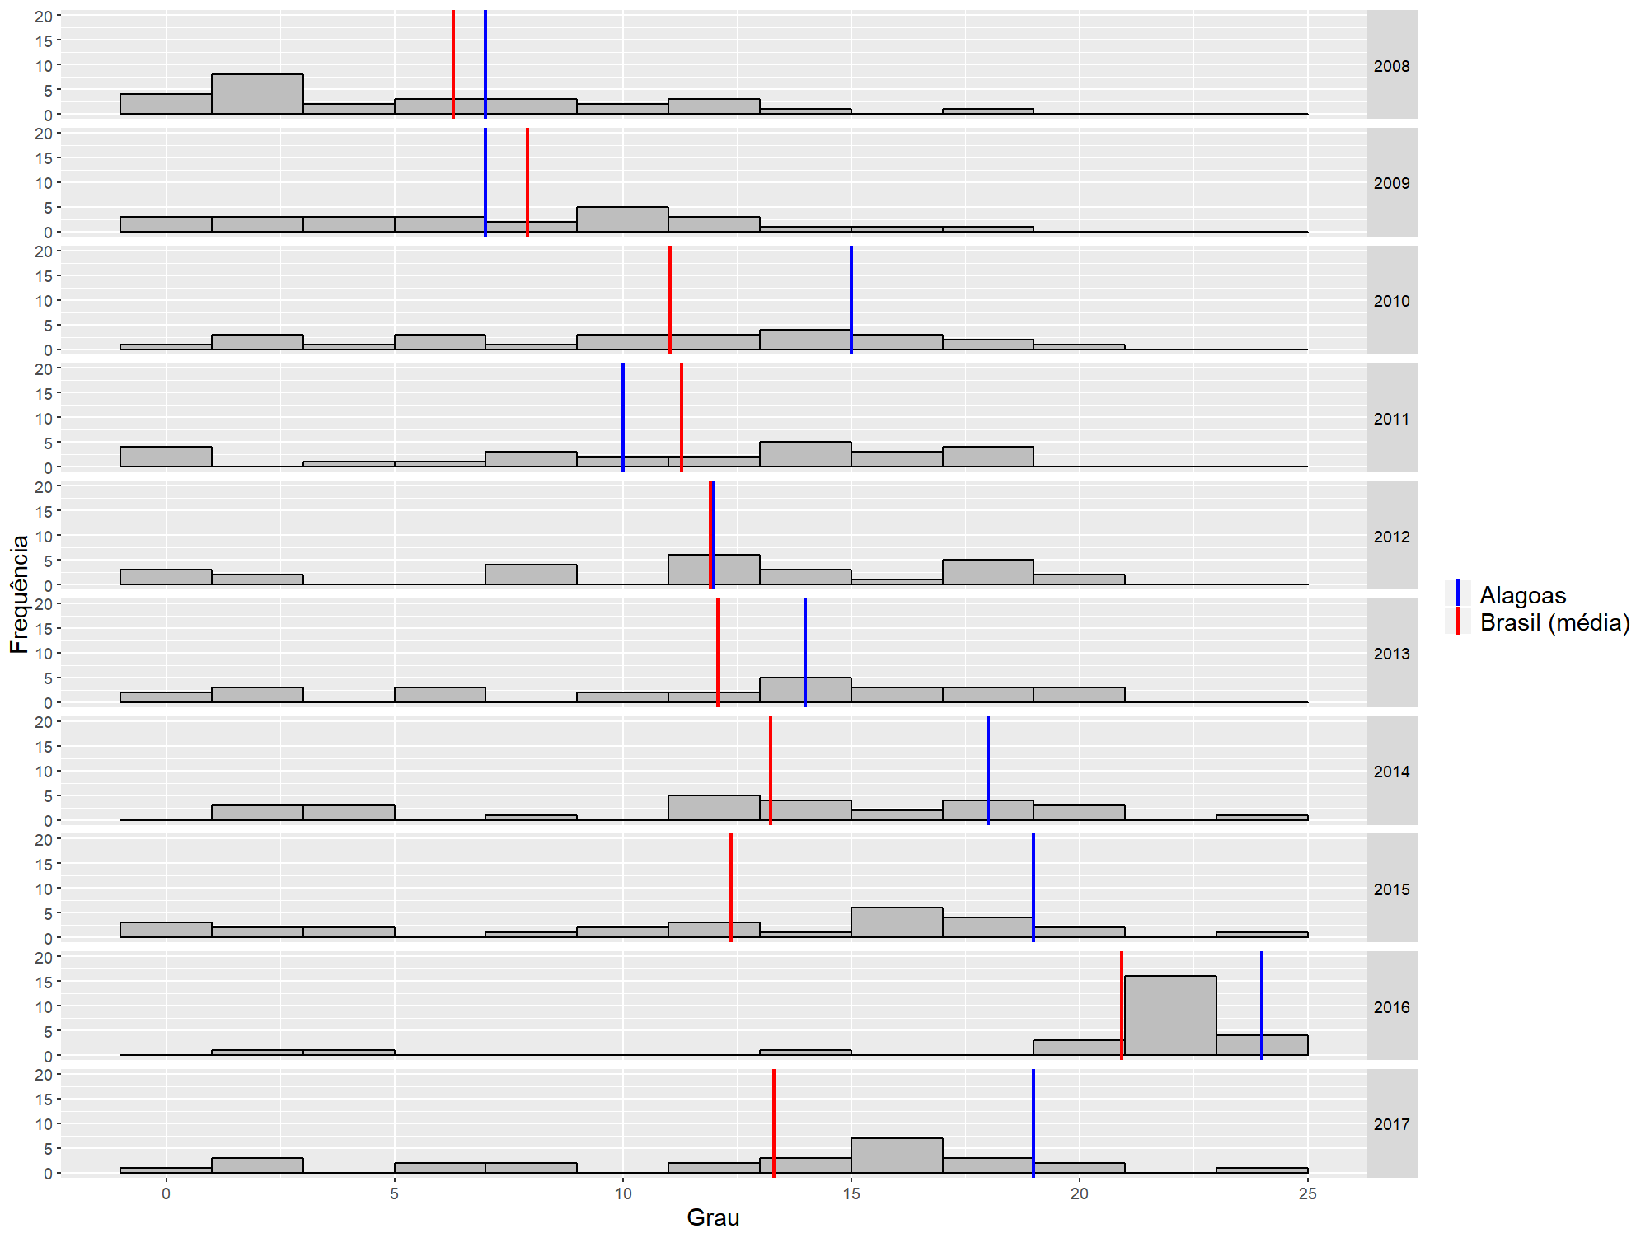
\includegraphics[scale=0.5]{Imagens/degree-hist.pdf}
	\caption{Histograma da Centralidade do Grau (\textit{Health Sciences})}
	\label{degree-health-hist-1}
\end{figure}

\begin{figure}[H]
	\centering
	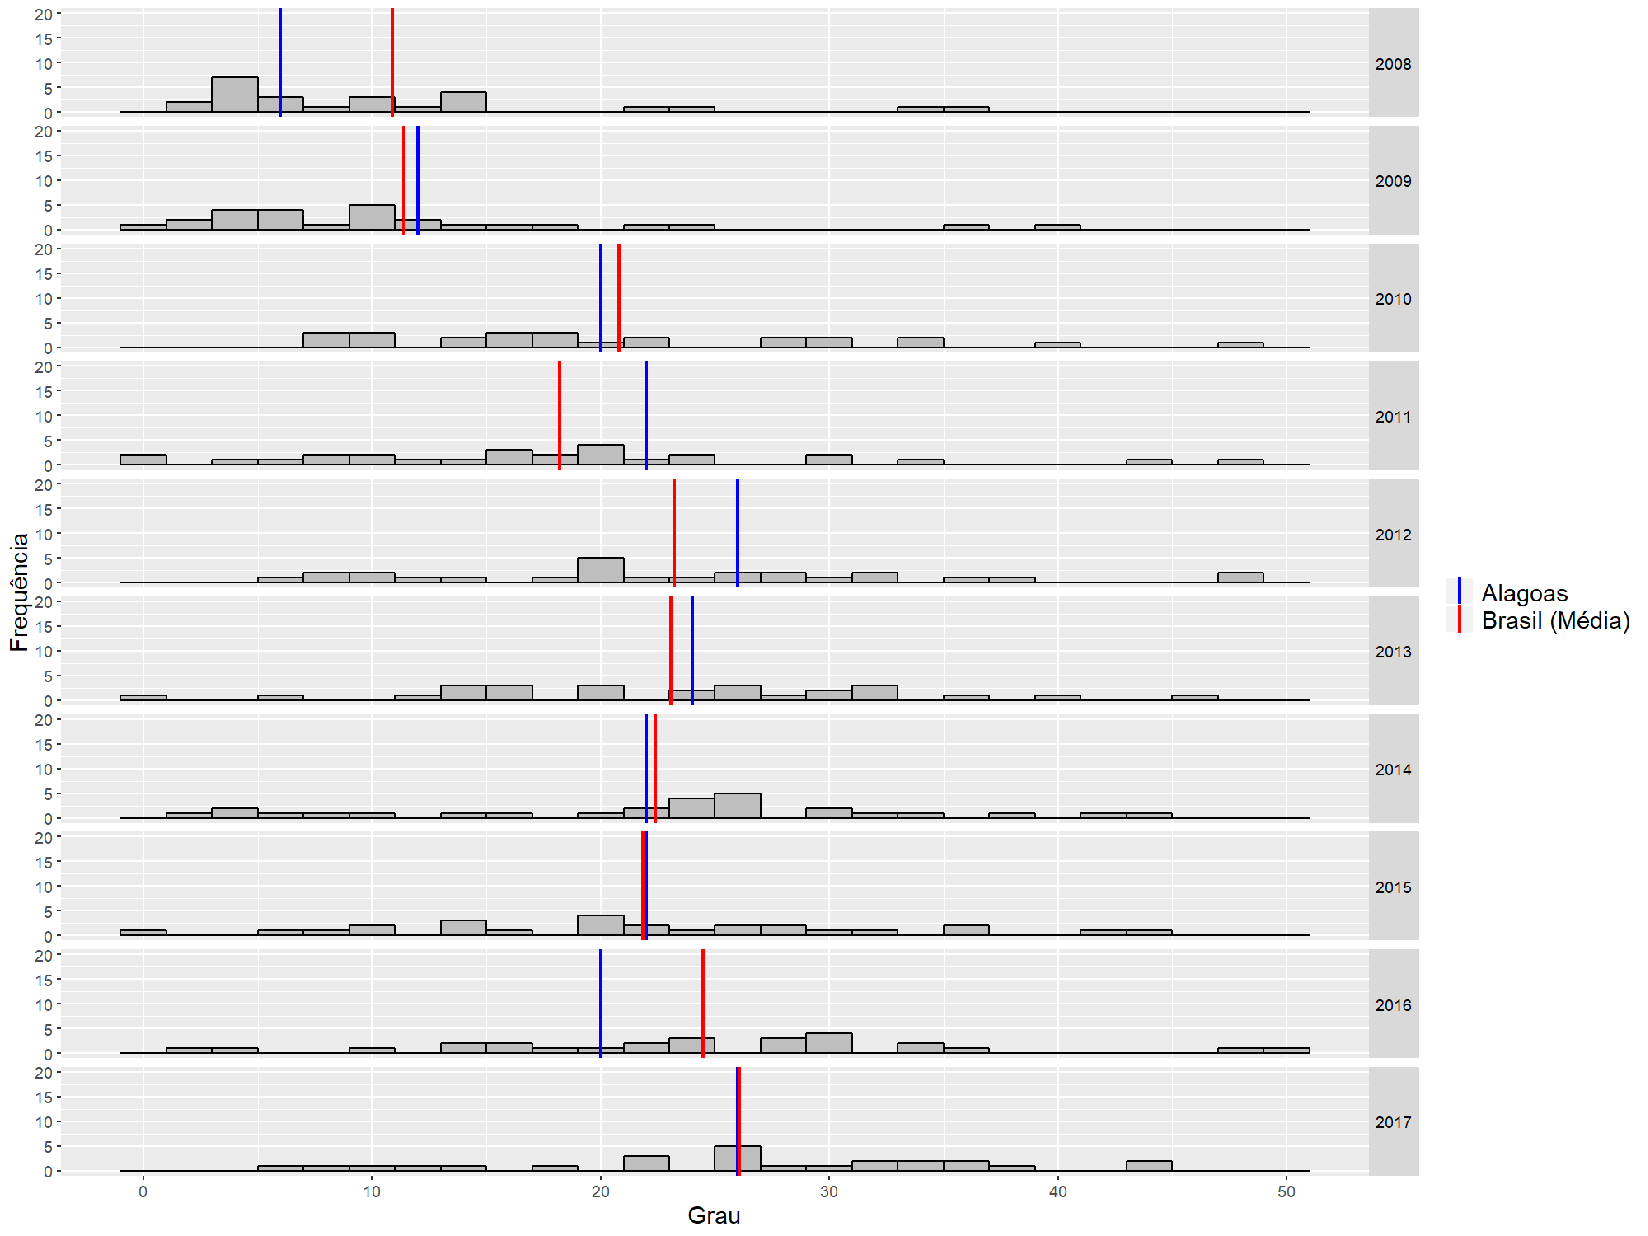
\includegraphics[scale=0.5]{Imagens/agricultural/degree-hist.pdf}
	\caption{Histograma da Centralidade do Grau (\textit{Agricultural Sciences})}
	\label{degree-agri-hist-1}
\end{figure}

\begin{figure}[H]
	\centering
	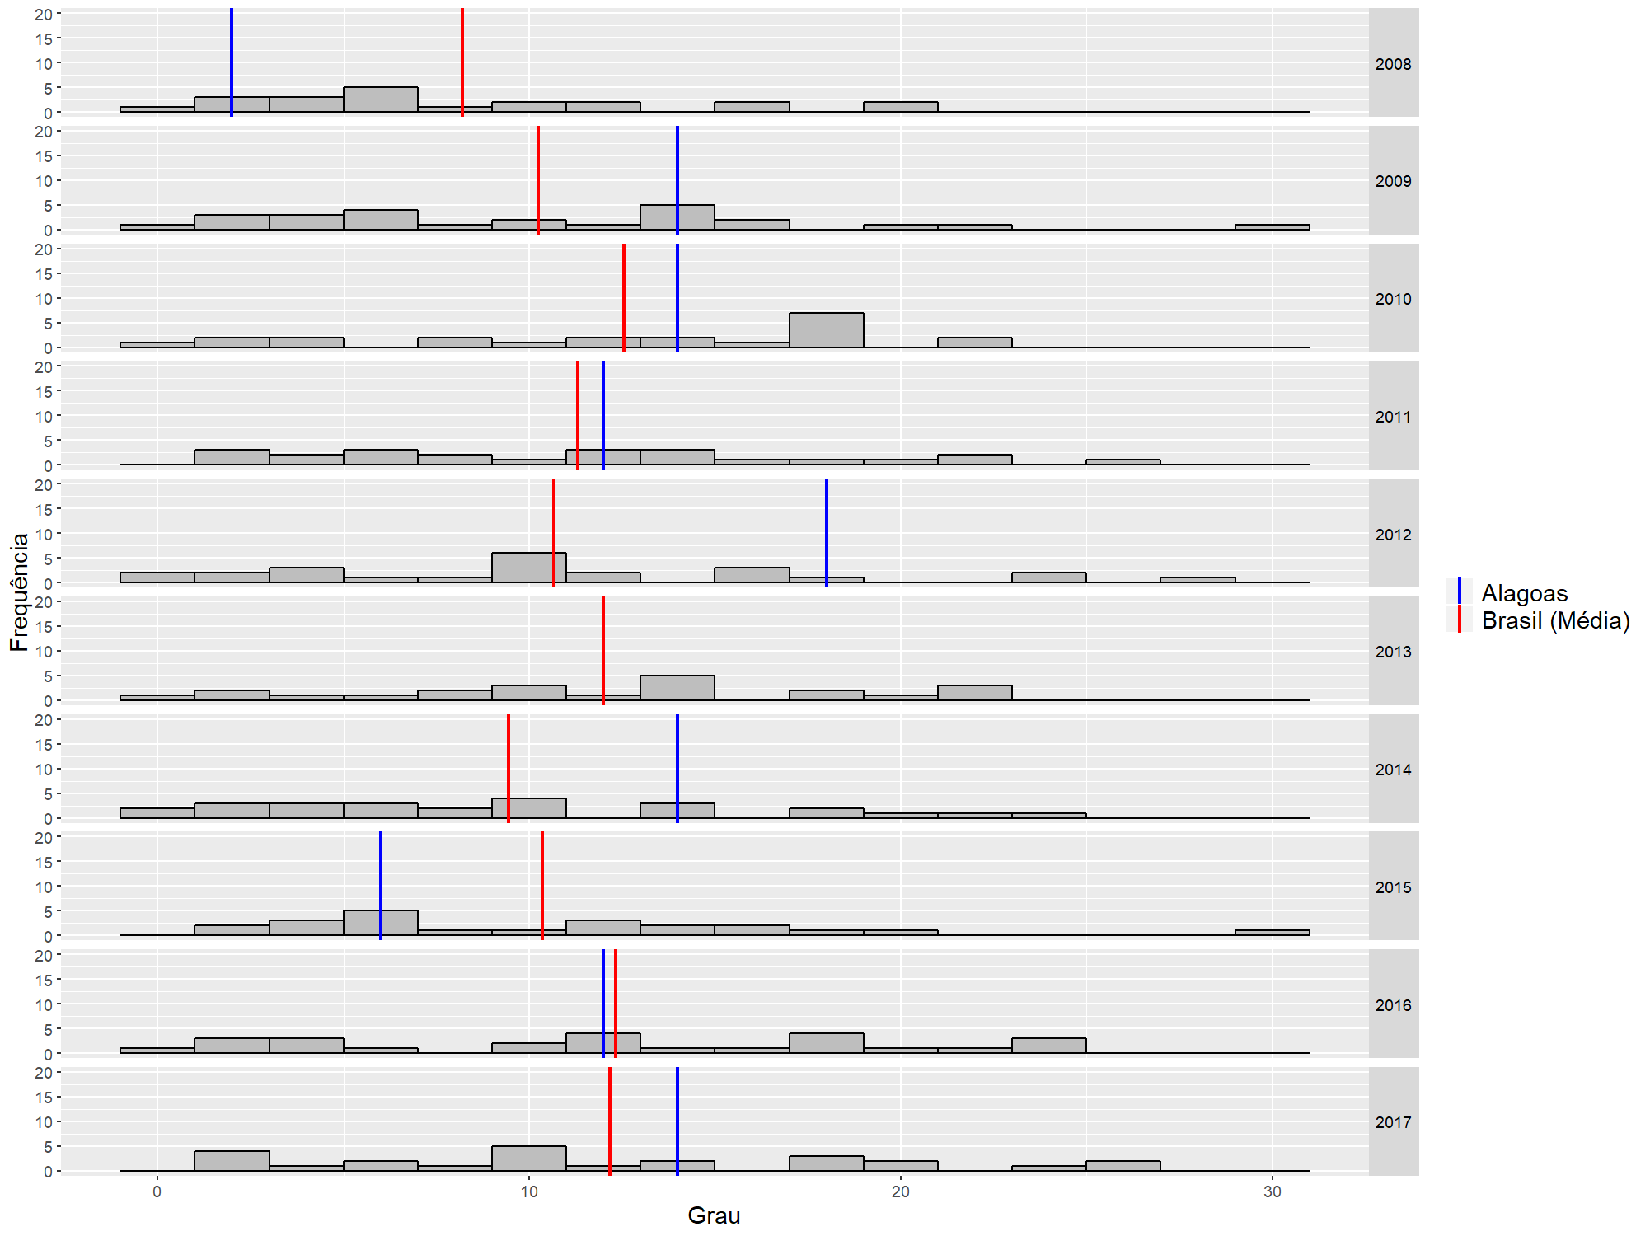
\includegraphics[scale=0.5]{Imagens/exact/degree-hist.pdf}
	\caption{Histograma da Centralidade do Grau (\textit{Exact and Earth Sciences})}
	\label{degree-exact-hist-1}
\end{figure}


O histograma \ref{degree-health-hist-1} indica a distribuição da medida de centralidade do grau para área de \textit{Health Sciences}, maneira a qual percebemos uma grande frequência no ano de 2016, em virtude da clusterização observada na tabela \ref{estruturais}, corroborando os anos que Alagoas (linha azul) esteve a frente neste marcador quando comparado a média do Brasil.

Na figura \ref{degree-agri-hist-1} observamos um posicionamento muito próximo da média da Rede Brasil (linha vermelha) e Alagoas (linha azul), e que exceto nos primeiro anos de 2008 a 2009 a distribuição concentrou-se na região central, de forma que muitos vértices obtiveram índices parecidos, exceto \textit{outliers} que estão presente em cada ano, dos quais podemos verificar na matriz \ref{matriz-agri} e no ranking apresentando em seção abaixo.

O histograma, figura \ref{degree-exact-hist-1} da área de \textit{Exact and Earth Sciences} mostra o posicionamento da centralidade do grau de Alagoas acima do Brasil, e uma distribuição dos índices aferidos mais dispersos.

%%% CLOSENESS

\subsection{\textbf{Centralidade de Proximidade}}

A figura \ref{closeness-tab} apresenta os resultados da medida de centralidade de proximidade em relação a Rede Brasil (média) e Alagoas, para todas as áreas. Essa medida indica quão próximo um vértice encontra-se um do outro, considerando seu posicionamento na rede. Indicando assim o seu papel de influência e importância pelo aspecto da proximidade.


\begin{table}[H]
	\centering
	\begin{tabular}{|c|l|l|l|l|l|l|}
		\hline
		\multicolumn{7}{|c|}{\textbf{\begin{tabular}[c]{@{}c@{}}Centralidade de Proximidade  \\ (Closeness Centrality) por Área\end{tabular}}}                                                                                                                                                                                                                                                  \\ \hline
		\rowcolor[HTML]{C0C0C0} 
		\textbf{Ano}    & \multicolumn{2}{|c|}{\cellcolor[HTML]{C0C0C0}\textbf{\begin{tabular}[c]{@{}c@{}}Health \\ Sciences\end{tabular}}} & \multicolumn{2}{|c|}{\cellcolor[HTML]{C0C0C0}\textbf{\begin{tabular}[c]{@{}c@{}}Agricultural \\ Sciences\end{tabular}}} & \multicolumn{2}{c|}{\cellcolor[HTML]{C0C0C0}\textbf{\begin{tabular}[c]{@{}c@{}}Exact and \\ Earth Sciences\end{tabular}}} \\ \hline
		\rowcolor[HTML]{EFEFEF} 
		\textbf{Rede}   & \textbf{Brasil}                                        & \textbf{Alagoas}                                        & \textbf{Brasil}                                           & \textbf{Alagoas}                                           & \textbf{Brasil}                                             & \textbf{Alagoas}                                            \\ \hline
		2008            & 0,5303                                                 & 0,5434                                                  & 0,5414                                                    & 0,4528                                                     & 0,4824                                                      & 0,3333                                                      \\ \hline
		2009            & 0,5789                                                 & 0,5609                                                  & 0,5543                                                    & 0,5455                                                     & 0,4978                                                      & 0,5610                                                       \\ \hline
		2010            & 0,6772                                                 & 0,7419                                                  & 0,6531                                                    & 0,6316                                                     & 0,5435                                                      & 0,5263                                                      \\ \hline
		2011            & 0,6699                                                 & 0,6216                                                  & 0,6444                                                    & 0,6487                                                     & 0,5216                                                      & 0,5366                                                      \\ \hline
		2012            & 0,6700                                                   & 0,6666                                                  & 0,6663                                                    & 0,6757                                                     & 0,5400                                                        & 0,6000                                                         \\ \hline
		2013            & 0,6852                                                 & 0,7058                                                  & 0,6747                                                    & 0,6667                                                     & 0,5544                                                      & 0,5556                                                      \\ \hline
		2014            & 0,6957                                                 & 0,7812                                                  & 0,6312                                                    & 0,6191                                                     & 0,5033                                                      & 0,5641                                                      \\ \hline
		2015            & 0,6697                                                 & 0,7812                                                  & 0,6676                                                    & 0,6487                                                     & 0,5306                                                      & 0,5122                                                      \\ \hline
		2016            & 0,8788                                                 & 0,9615                                                  & 0,6780                                                     & 0,6250                                                      & 0,5206                                                      & 0,5111                                                      \\ \hline
		2017            & 0,6993                                                 & 0,8064                                                  & 0,6995                                                    & 0,6857                                                     & 0,5267                                                      & 0,5750                                                       \\ \hline
	\end{tabular}
\caption{Medidas de Centralidade de Proximidade por Área (2008-2017)}
\label{closeness-tab}
\end{table}


\subsubsection{Health Sciences}

\begin{figure}[H]
	\centering
	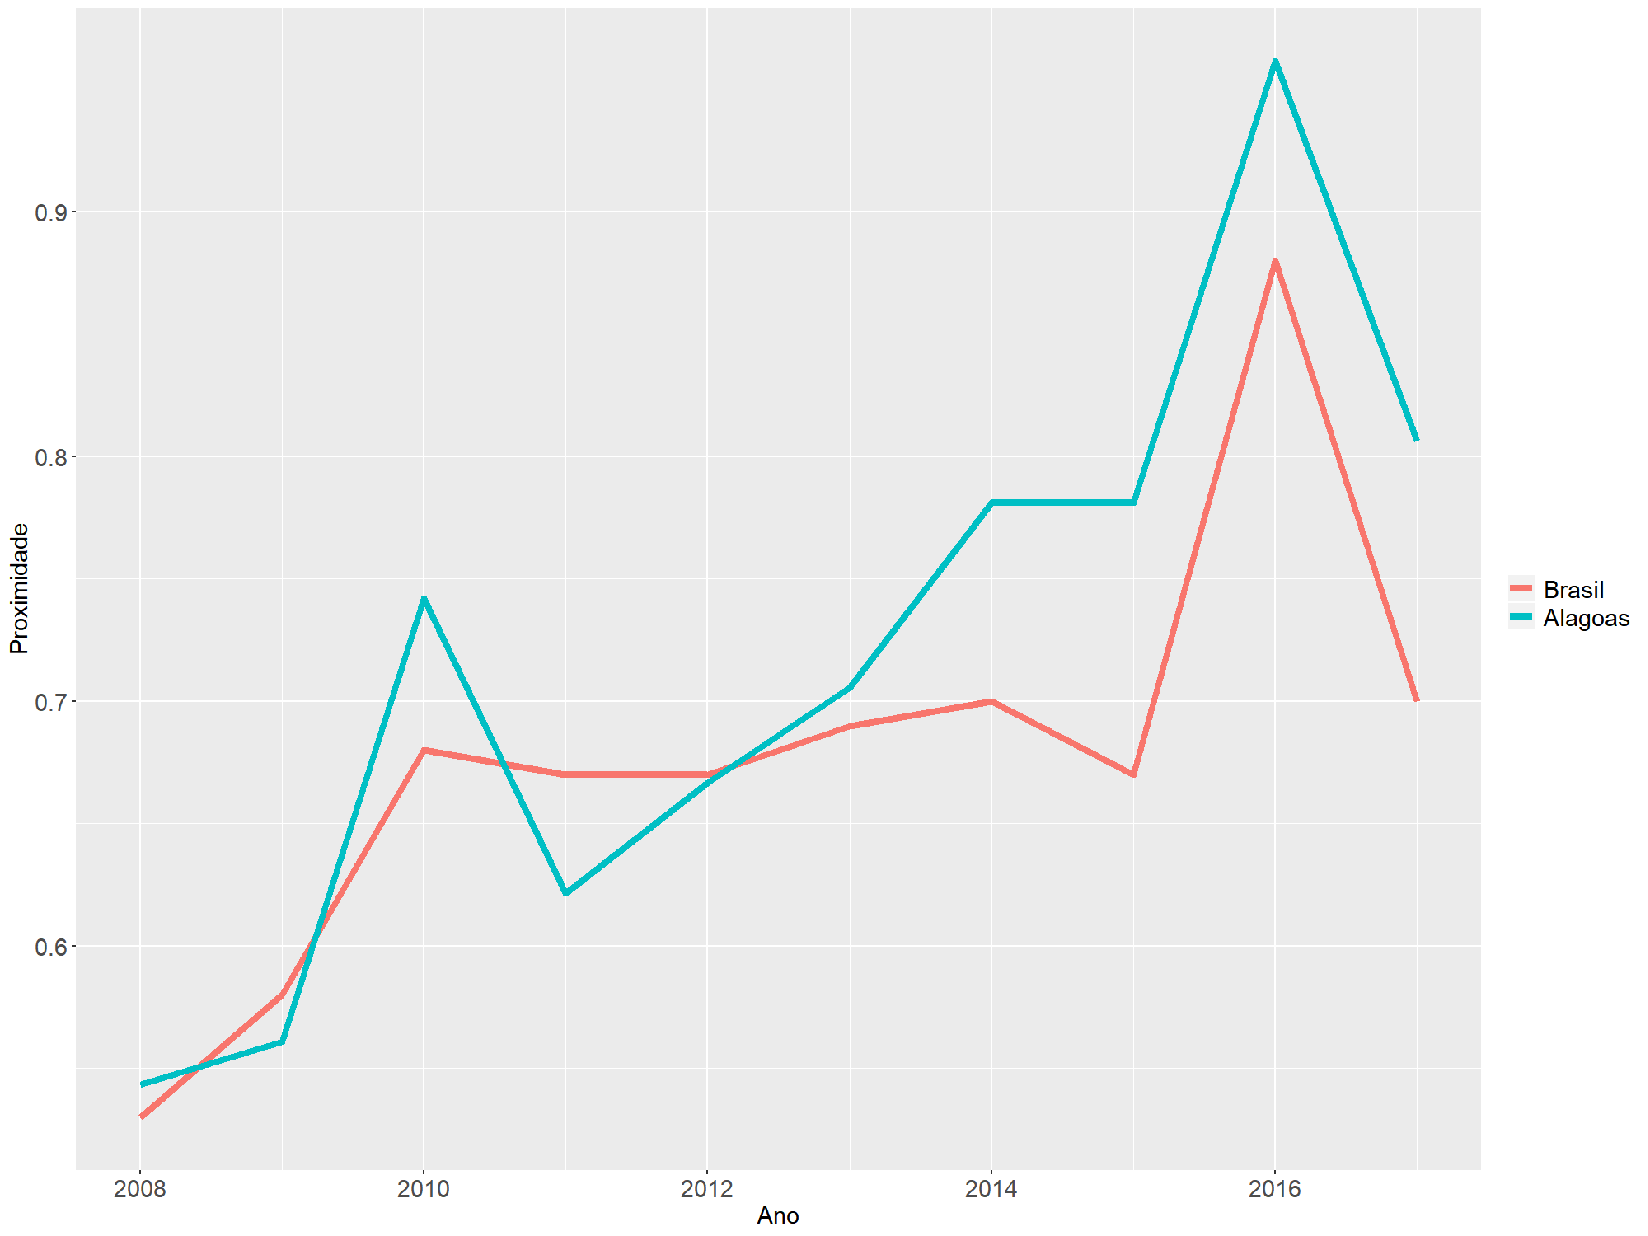
\includegraphics[scale=0.4]{Imagens/graf-linha-closeness-br-al.pdf}
	\caption{Centralidade de Proximidade (\textit{Health Sciences})}
	\label{close-health-1}
\end{figure}

\subsubsection{Agricultural Sciences}

\begin{figure}[H]
	\centering
	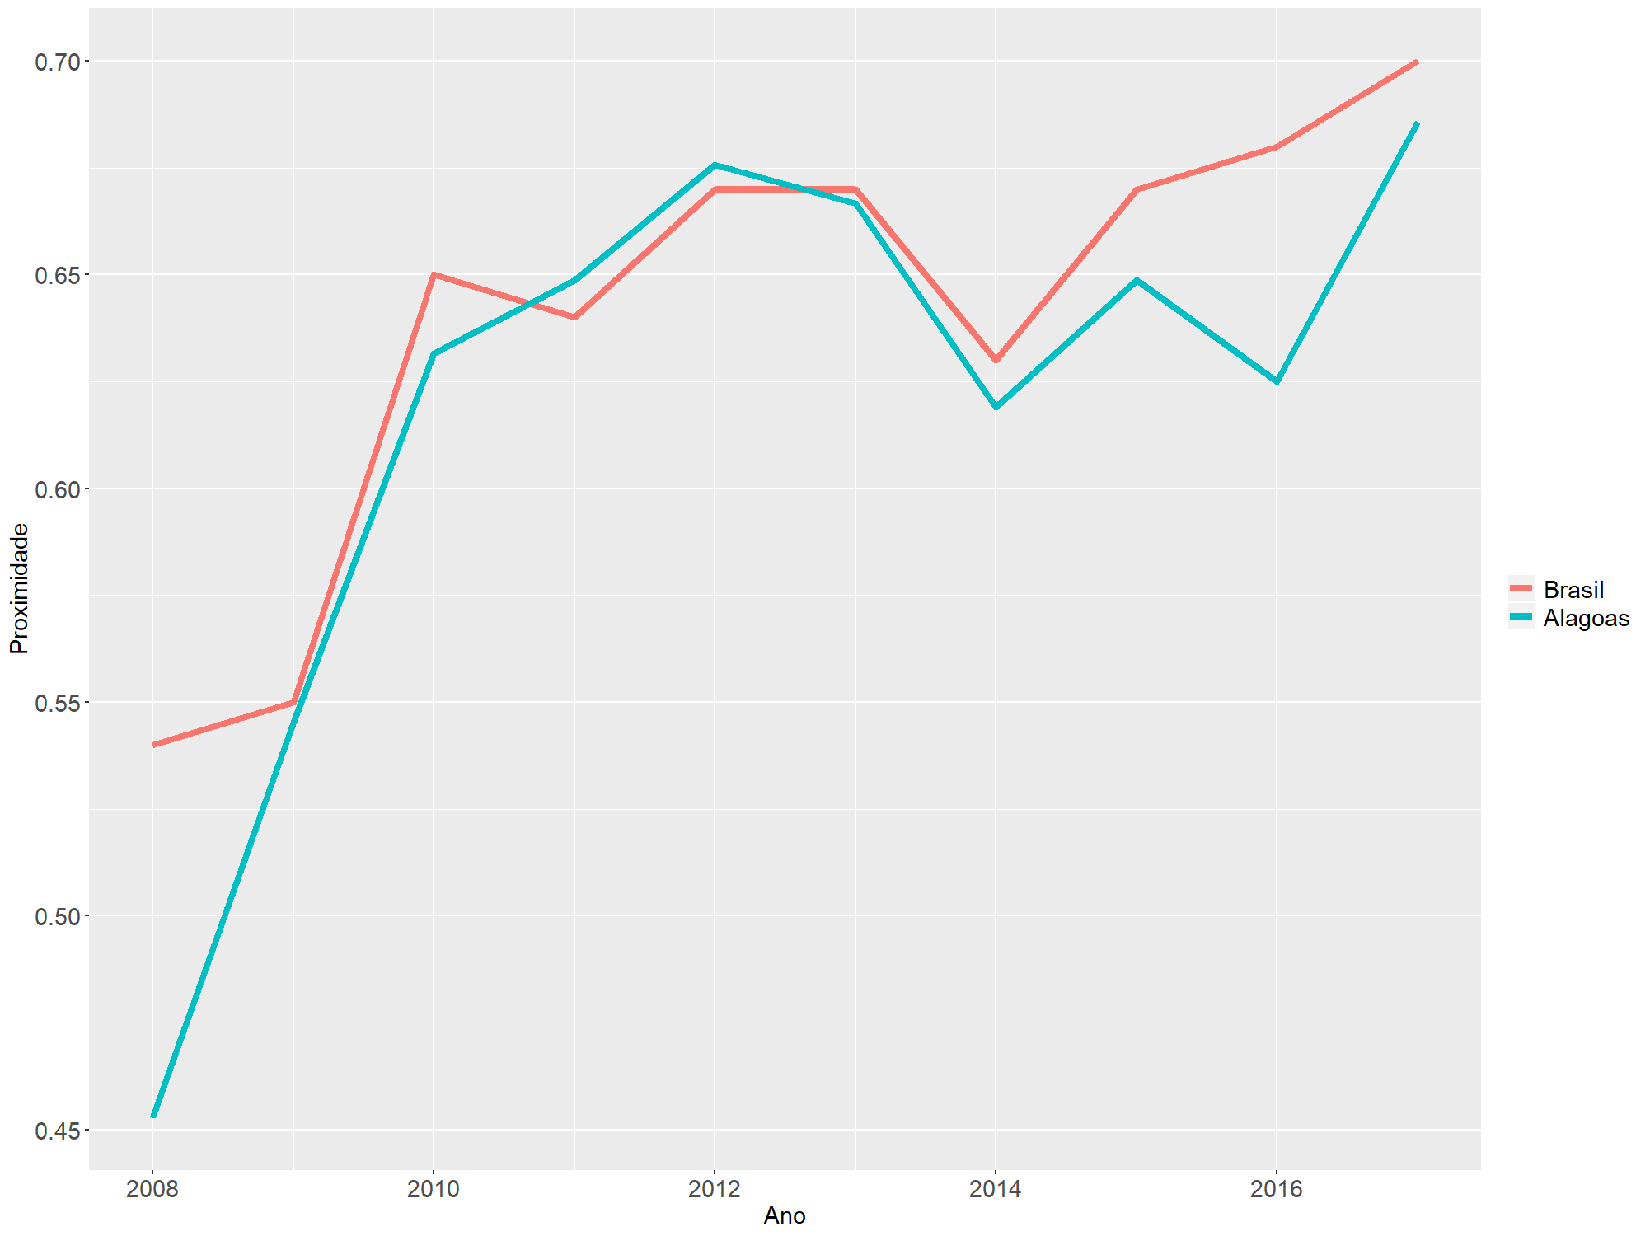
\includegraphics[scale=0.4]{Imagens/agricultural/graf-linha-closeness-br-al.pdf}
	\caption{Centralidade de Proximidade (\textit{Agricultural Sciences})}
	\label{close-agri-1}
\end{figure}

\subsubsection{Exact and Earth Sciences}

\begin{figure}[H]
	\centering
	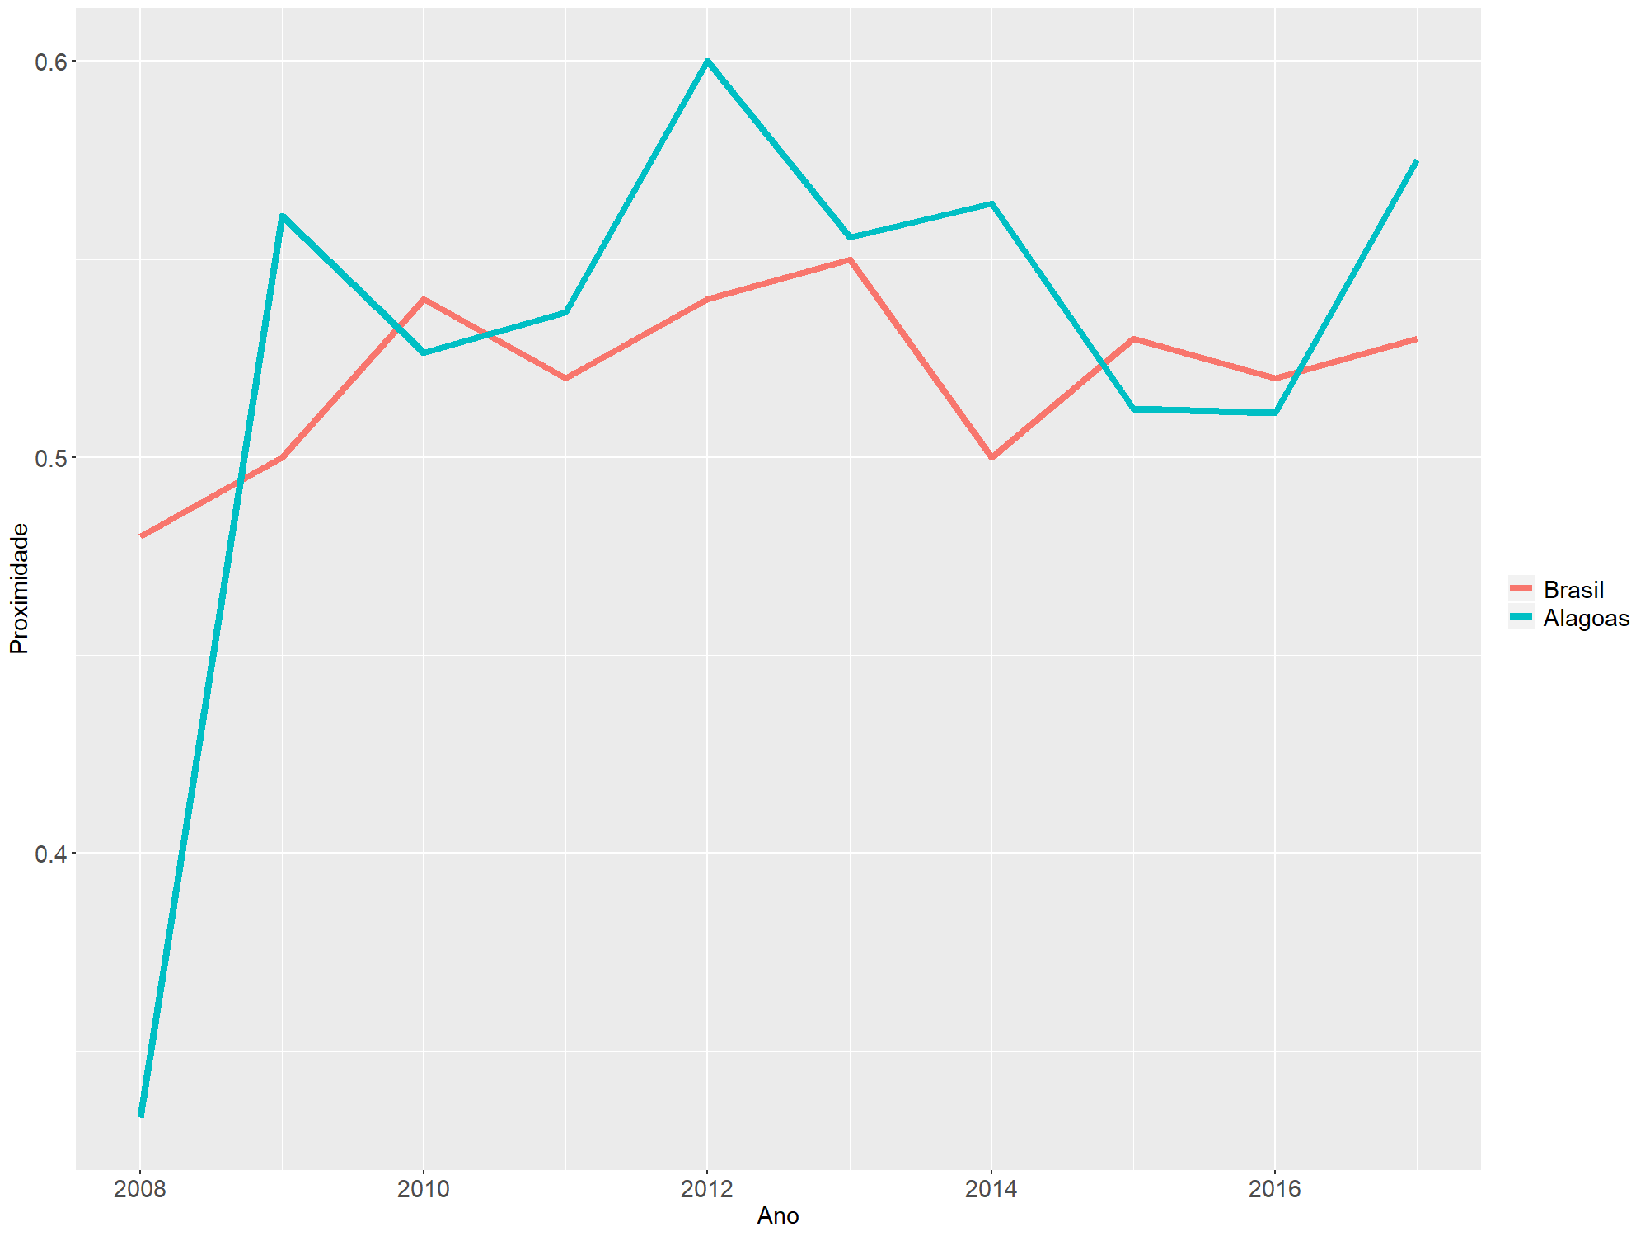
\includegraphics[scale=0.4]{Imagens/exact/graf-linha-closeness-br-al.pdf}
	\caption{Centralidade de Proximidade (\textit{Exact and Earth Sciences})}
	\label{close-exact-1}
\end{figure}

As curvas da Rede Brasil (vermelha) e Alagoas (azul), também se projetaram em sentidos análogos, destaque que na área de \textit{Health Sciences} conforme \ref{close-health-1} que exceto nos anos 2009 e 2011 em todo o período manteve-se acima da média do Brasil. 

Na área de \textit{Agricultural Science} conforme figura \ref{close-agri-1}, os resultados foram muito próximos, resultando que Alagoas ficou em que alguns anos abaixo da média, como vimos na figura da Matriz de Coautoria \ref{matriz-agri} e o que será corroborado pelo ranking apresentado abaixo, pelo destaque dos estados do Rio Grande do Sul e Rio Grande do Norte em Ciências Agrárias.

Na análise gráfica da centralidade de proximidade da área \textit{Exact and Earth Sciences}, verificamos um baixo índice aferido por Alagoas no ano de 2008 e que a partir de 2009 seguiu em patamar superior a média do Brasil, tendo sido a área de maior destaque para medidade de centralidade da proximidade.


\subsubsection{Health Sciences}

\begin{figure}[H]
	\centering
	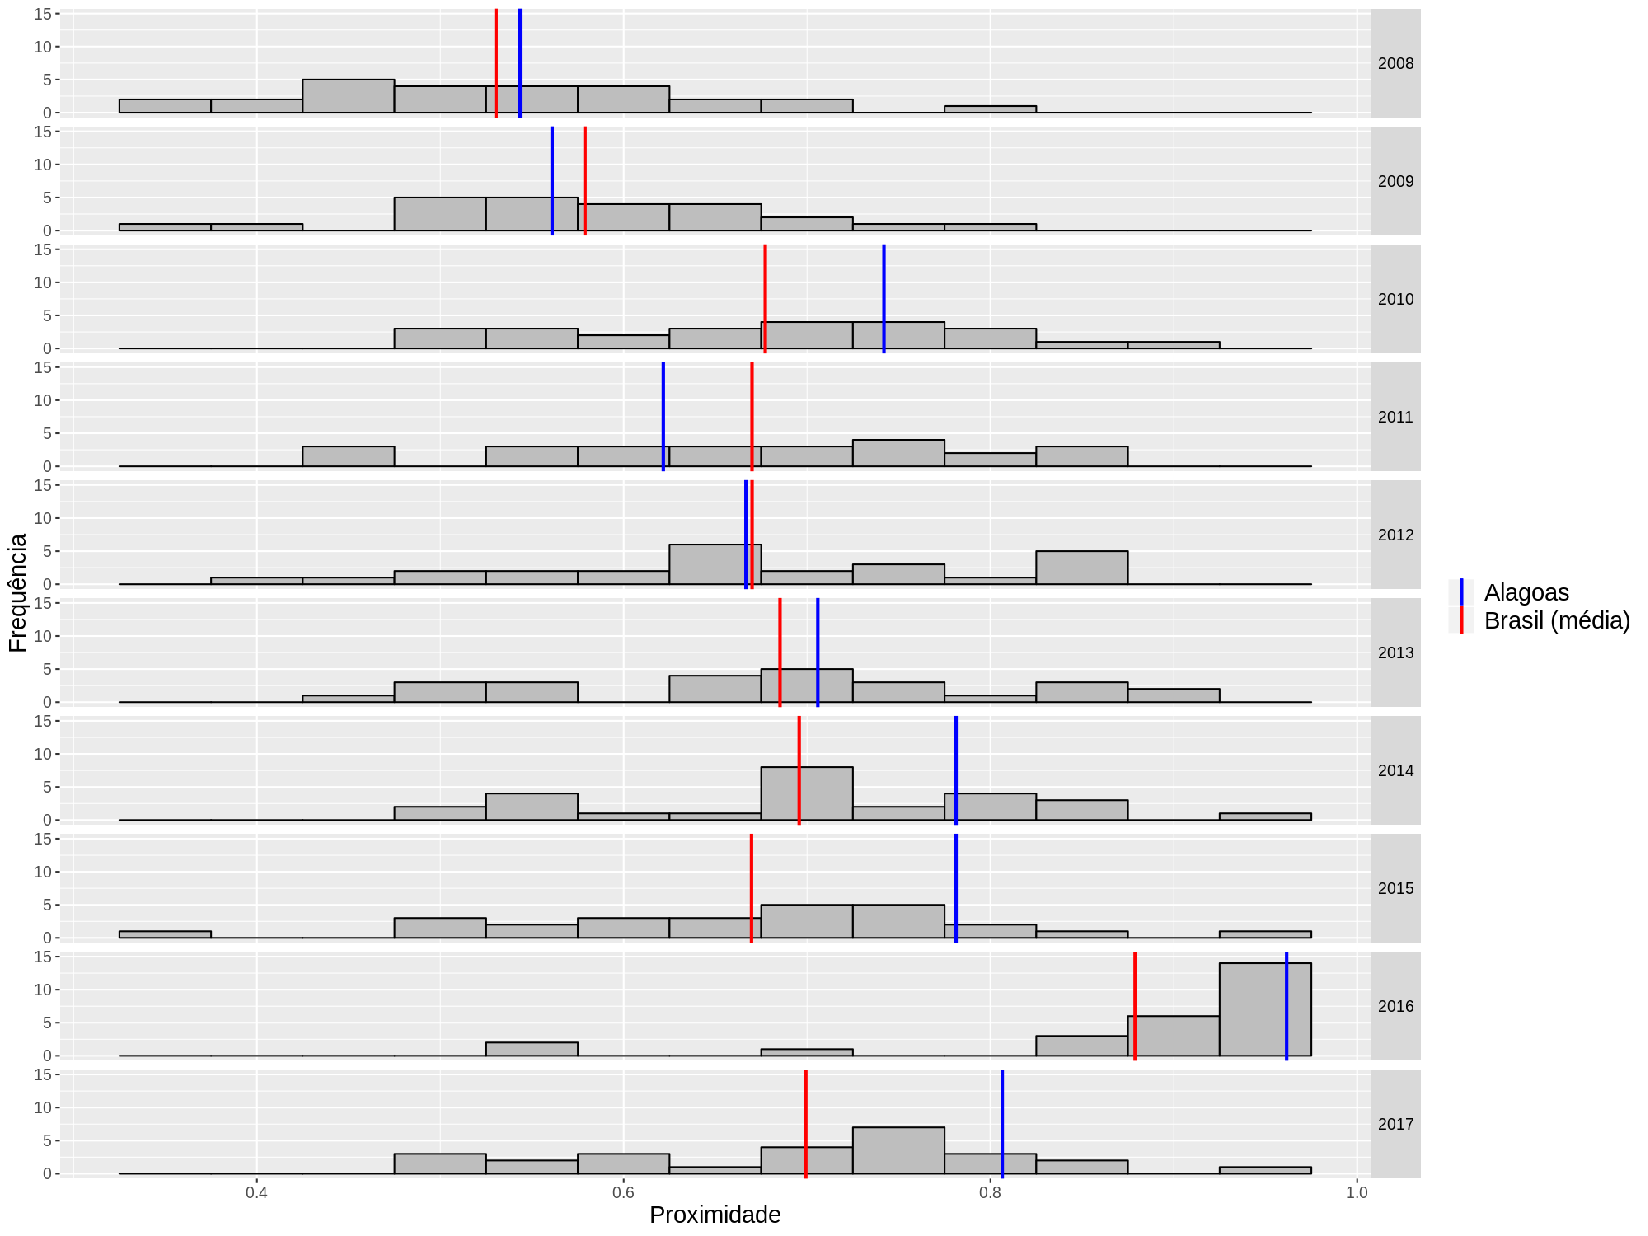
\includegraphics[scale=0.5]{Imagens/closeness-hist.pdf}
	\caption{Histograma da Centralidade de Proximidade (\textit{Health Sciences})}
	\label{hist-health-close-1}
\end{figure}

\subsubsection{Agricultural Sciences}

\begin{figure}[H]
	\centering
	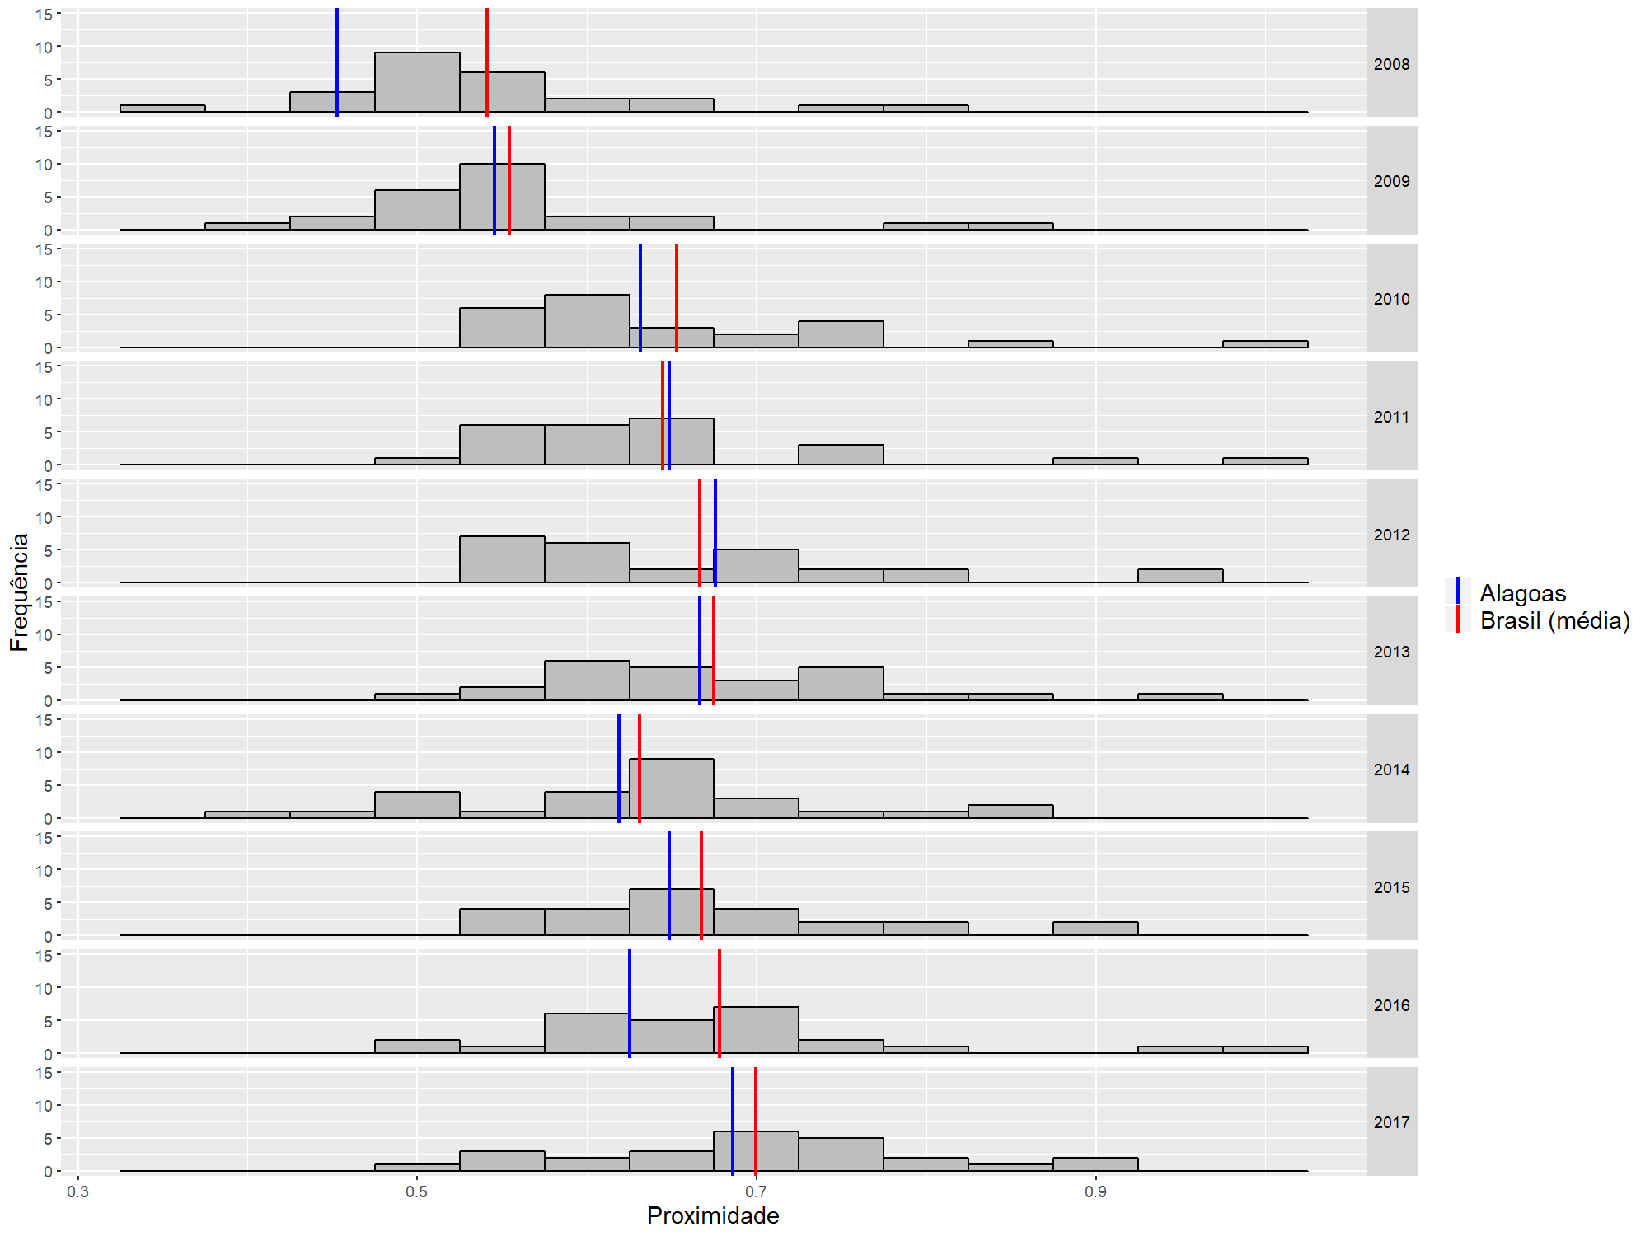
\includegraphics[scale=0.5]{Imagens/agricultural/closeness-hist.pdf}
	\caption{Histograma da Centralidade de Proximidade (\textit{Agricultural Sciences})}
	\label{hist-agri-close-1}
\end{figure}

\subsubsection{Exact and Earth Sciences}

\begin{figure}[H]
	\centering
	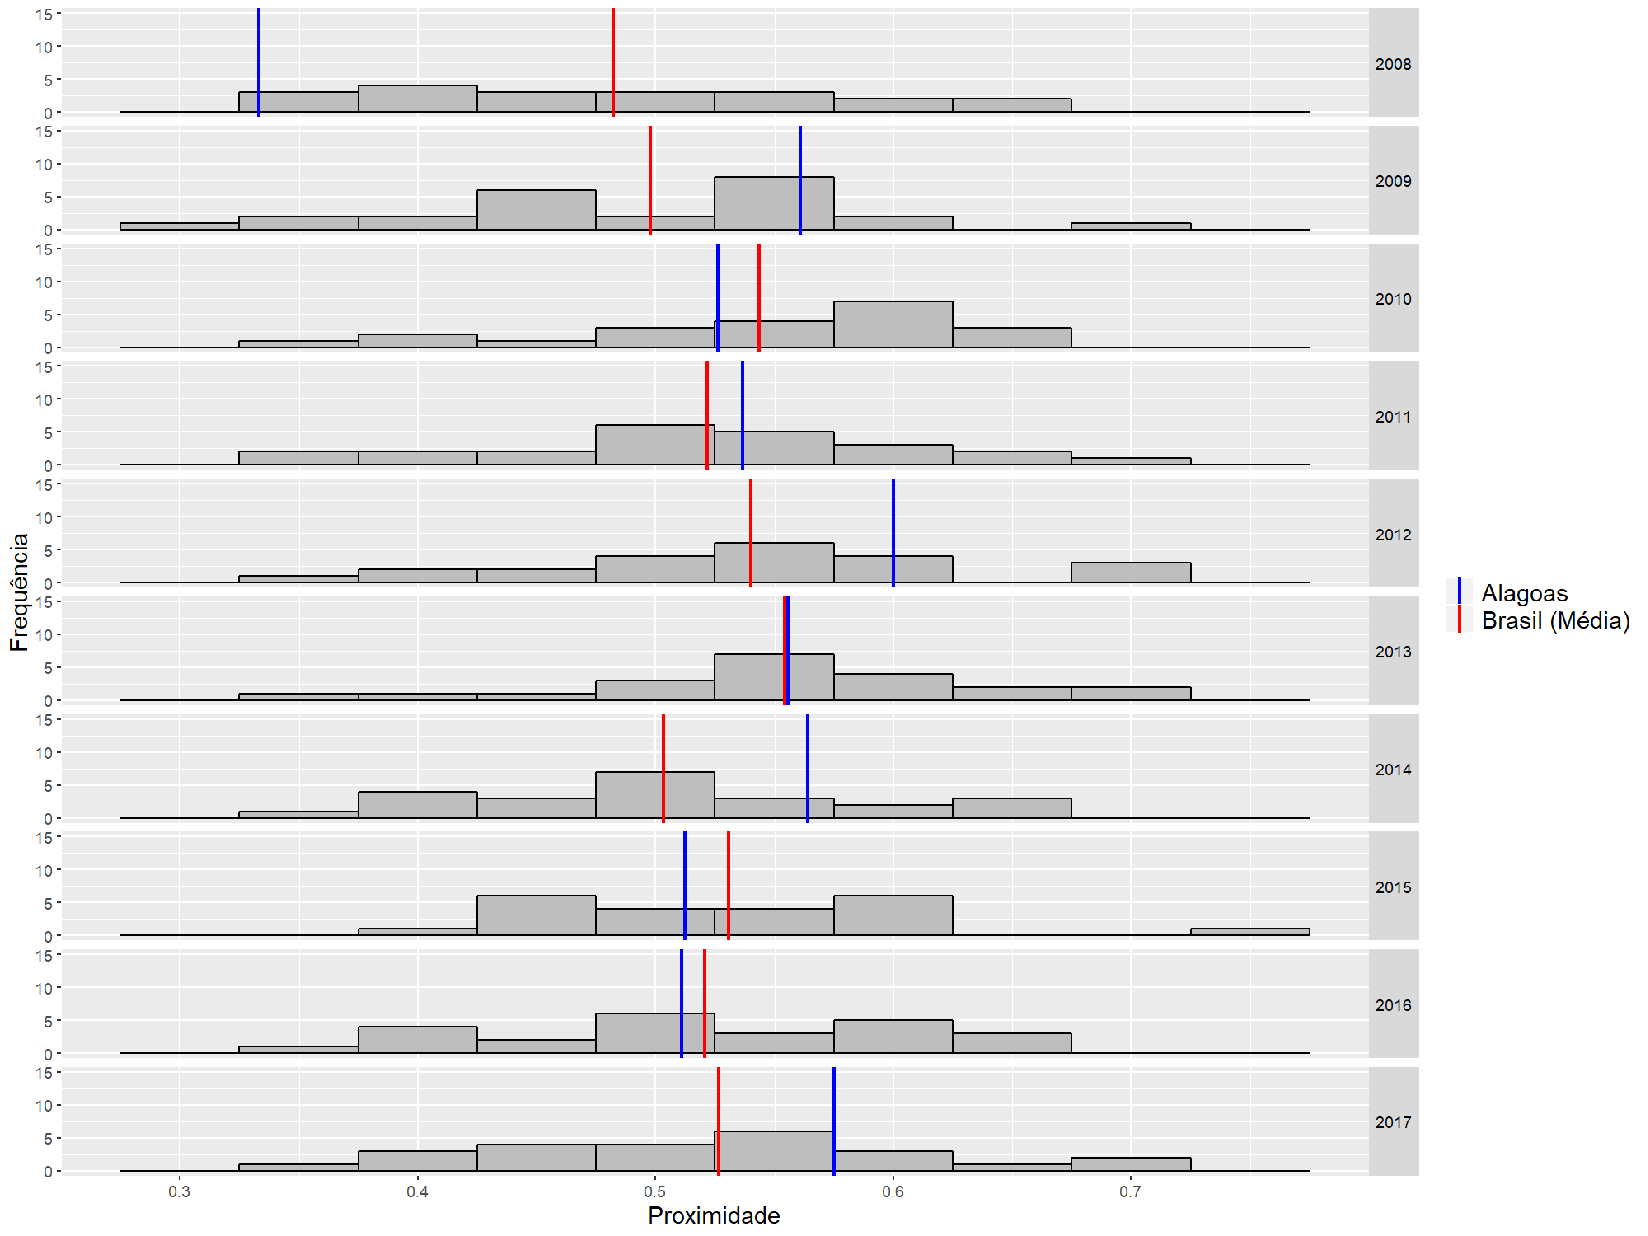
\includegraphics[scale=0.5]{Imagens/exact/closeness-hist.pdf}
	\caption{Histograma da Centralidade de Proximidade (\textit{Exact and Earth Sciences})}
	\label{hist-exact-close-1}
\end{figure}

As figuras \ref{hist-health-close-1}, apresenta o histograma de distribuição para a área de \textit{Health Sciences}, o qual podemos destacar ano de 2016, em que as frequências se concentraram em alto índice comparado aos demais anos, e que Alagoas ficou acima da média para essa medida desde o ano de 2013. Resultando que sua proximidade quando comparada a média dos vértices do Brasil é superior.

Em \textit{Agricultural Sciences}, visto pelo histograma na figura \ref{hist-agri-close-1}, a média do Brasil e Alagoas são marcados muito próximos no histograma que possui distribuição em todos anos muito central. De forma que esta medida não apresentou relevante informação nessa área.

O histograma \ref{hist-exact-close-1} apresenta uma distribuição de sua frequência mais espaçada, sendo observador o marcador de Alagoas muito baixo no ano de 2008, muito provável pelos poucos artigos indexados neste ano por autores Alagoanos na área de \textit{Exact and Earth Sciences}, mas que a partir de 2009 a proximidade de Alagoas com a média do Brasil, supera em 2011, 2012, 2014, e 2017,


%%% BETWEENESS

\subsection{\textbf{Centralidade de Intermediação}}

A figura \ref{betweeness-tab} apresenta os resultados da medida de centralidade de intermediação em relação a Rede Brasil (média) e Alagoas, para todas as áreas. Essa medida indica a capacidade de intermediação de um vértice a outro, considerando seu posicionamento na rede.

\begin{table}[H]
	\centering
	\begin{tabular}{|c|l|l|l|l|l|l|}
		\hline
		\multicolumn{7}{|c|}{\textbf{\begin{tabular}[c]{@{}c@{}}Centralidade de Intermediação\\ (Betweeness Centrality) por Área\end{tabular}}}                                                                                                                                                                                                                                                 \\ \hline
		\rowcolor[HTML]{C0C0C0} 
		\textbf{Ano}    & \multicolumn{2}{c|}{\cellcolor[HTML]{C0C0C0}\textbf{\begin{tabular}[c]{@{}c@{}}Health \\ Sciences\end{tabular}}} & \multicolumn{2}{c|}{\cellcolor[HTML]{C0C0C0}\textbf{\begin{tabular}[c]{@{}c@{}}Agricultural \\ Sciences\end{tabular}}} & \multicolumn{2}{c|}{\cellcolor[HTML]{C0C0C0}\textbf{\begin{tabular}[c]{@{}c@{}}Exact and \\ Earth Sciences\end{tabular}}} \\ \hline
		\rowcolor[HTML]{EFEFEF} 
		\textbf{Rede}   & \textbf{Brasil}                                        & \textbf{Alagoas}                                        & \textbf{Brasil}                                            & \textbf{Alagoas}                                          & \textbf{Brasil}                                             & \textbf{Alagoas}                                            \\ \hline
		2008            & 0,0370                                                  & 0,0100                                                    & 0,0400                                                       & 0,0047                                                    & 0,0476                                                      & 0,0021                                                      \\ \hline
		2009            & 0,0396                                                 & 0,0100                                                    & 0,0385                                                     & 0,0130                                                     & 0,0400                                                        & 0,1036                                                      \\ \hline
		2010            & 0,0388                                                 & 0,0400                                                    & 0,0400                                                       & 0,0138                                                    & 0,0455                                                      & 0,0251                                                      \\ \hline
		2011            & 0,0400                                                   & 0,0100                                                    & 0,0370                                                      & 0,0154                                                    & 0,0435                                                      & 0,0153                                                      \\ \hline
		2012            & 0,0380                                                  & 0,0200                                                    & 0,0385                                                     & 0,0314                                                    & 0,0417                                                      & 0,1405                                                      \\ \hline
		2013            & 0,0384                                                 & 0,0600                                                    & 0,0385                                                     & 0,0289                                                    & 0,0455                                                      & 0,0424                                                      \\ \hline
		2014            & 0,0384                                                 & 0,0500                                                    & 0,0370                                                      & 0,0066                                                    & 0,0400                                                        & 0,0549                                                      \\ \hline
		2015            & 0,0370                                                  & 0,0400                                                    & 0,0385                                                     & 0,0088                                                    & 0,0455                                                      & 0,0037                                                      \\ \hline
		2016            & 0,0396                                                 & 0,1000                                                     & 0,0385                                                     & 0,0099                                                    & 0,0400                                                        & 0,0212                                                      \\ \hline
		2017            & 0,0369                                                 & 0,0400                                                    & 0,0400                                                       & 0,0216                                                    & 0,0417                                                      & 0,0274                                                      \\ \hline
	\end{tabular}
\caption{Medidas de Centralidade de Intermediação por Área (2008-2017)}
\label{betweeness-tab}
\end{table}

\subsubsection{Health Sciences}

\begin{figure}[H]
	\centering
	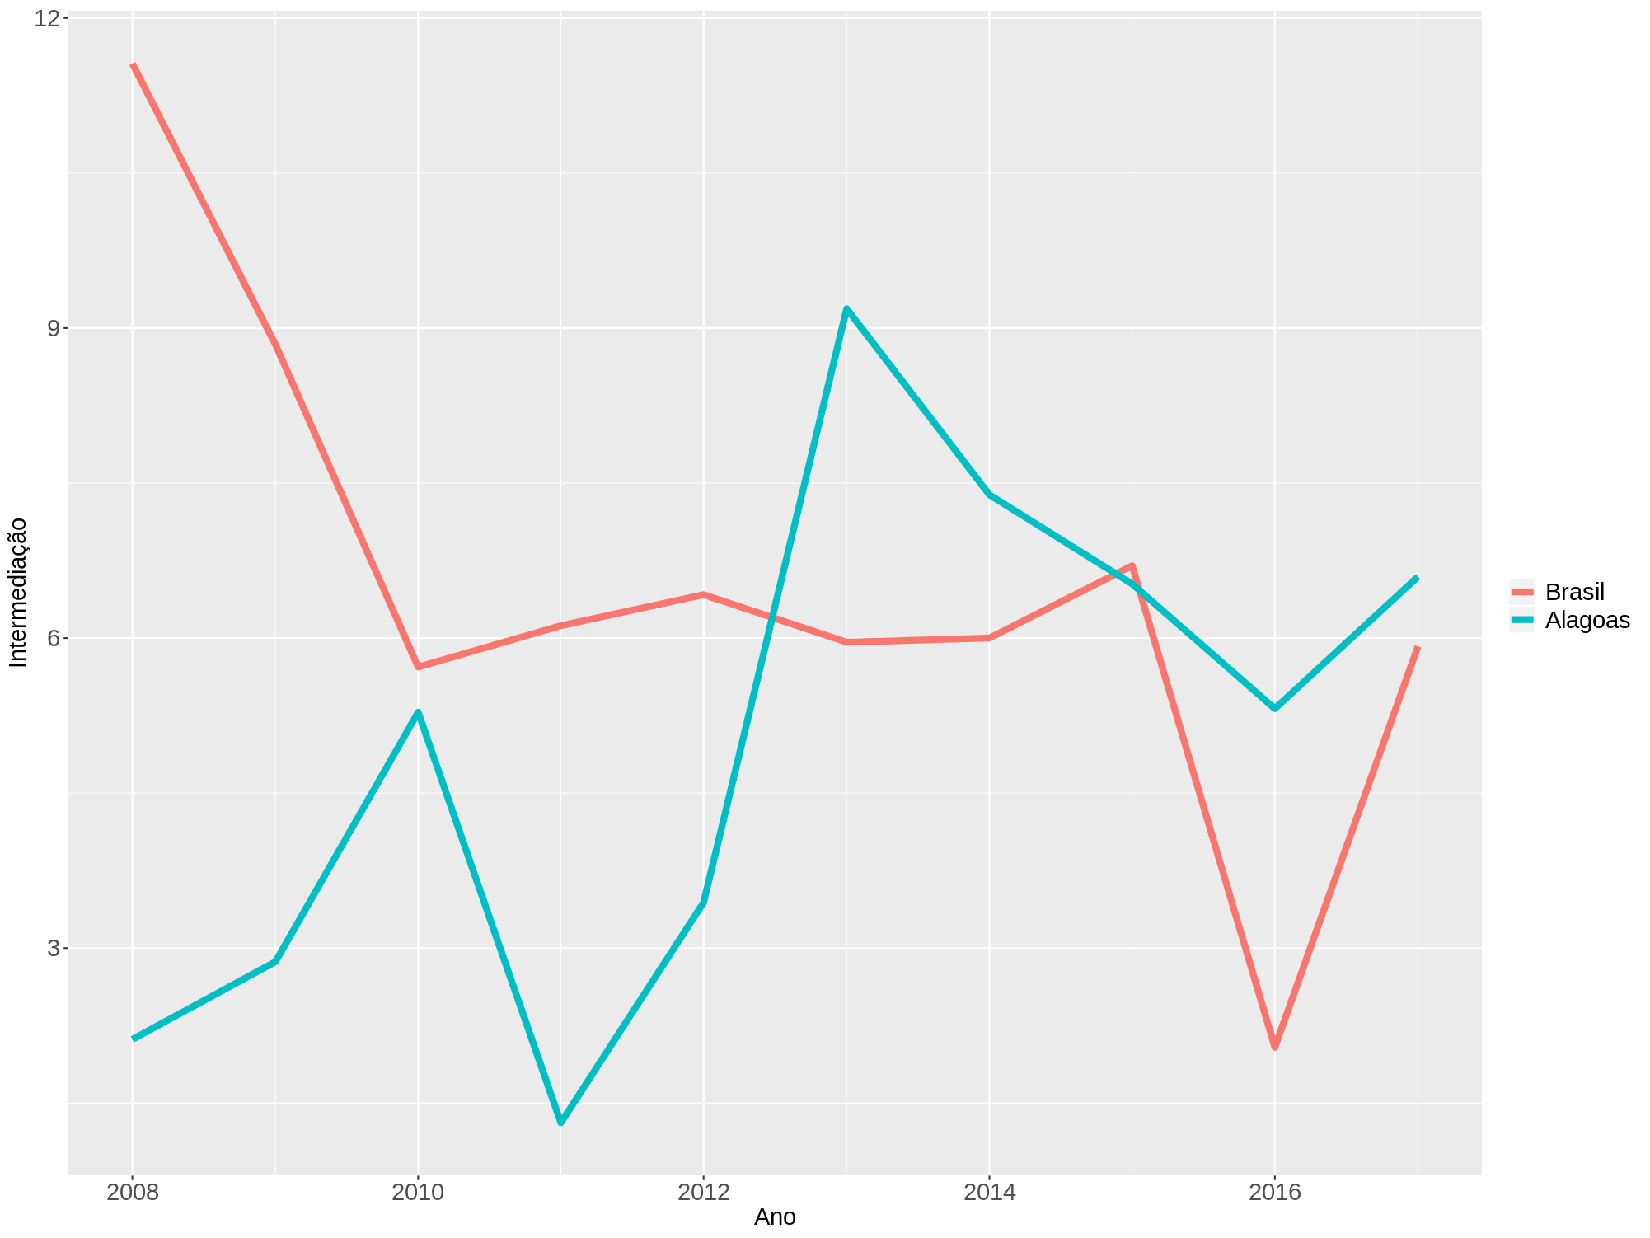
\includegraphics[scale=0.4]{Imagens/graf-linha-betweeness-br-al.pdf}
	\caption{Centralidade de Proximidade (\textit{Health Sciences})}
	\label{between-health-1}
\end{figure}

\subsubsection{Agricultural Sciences}

\begin{figure}[H]
	\centering
	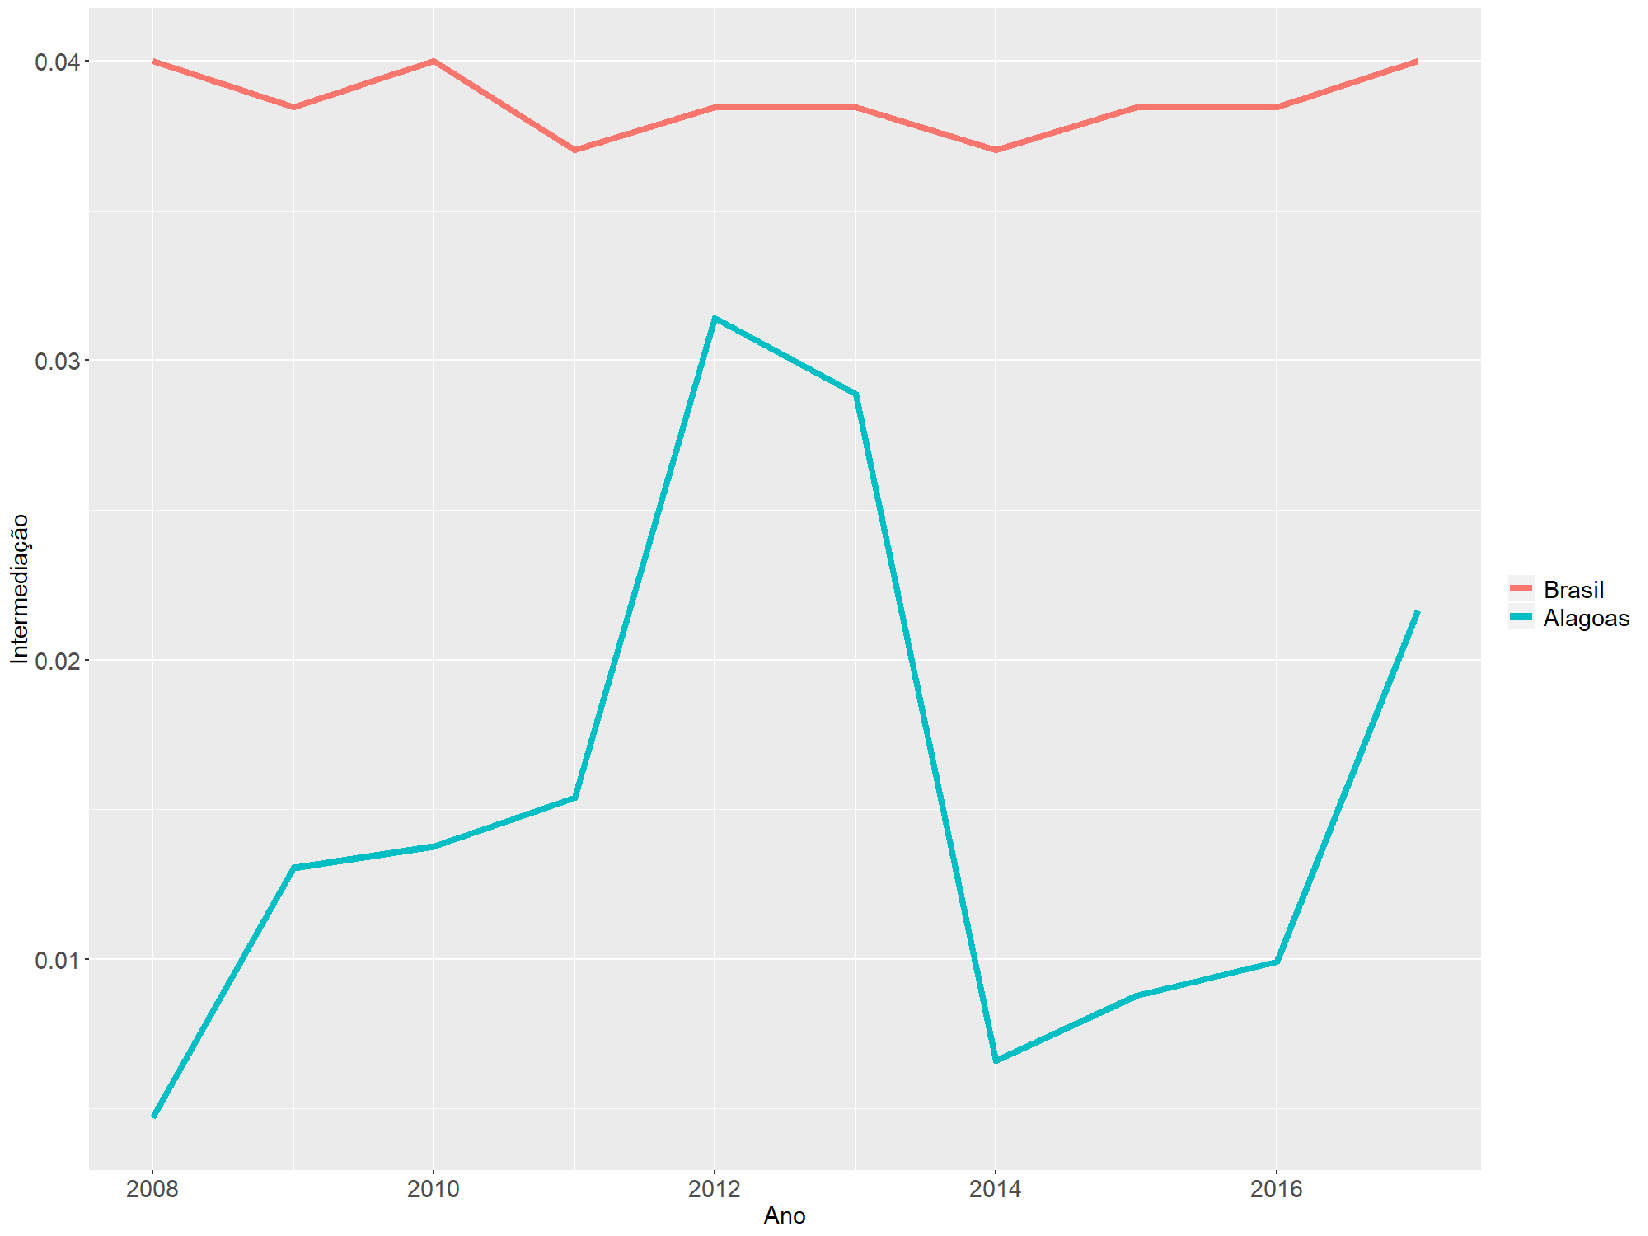
\includegraphics[scale=0.4]{Imagens/agricultural/graf-linha-betweeness-br-al.pdf}
	\caption{Centralidade de Proximidade (\textit{Agricultural Sciences})}
	\label{between-agri-1}
\end{figure}

\subsubsection{Exact and Earth Sciences}

\begin{figure}[H]
	\centering
	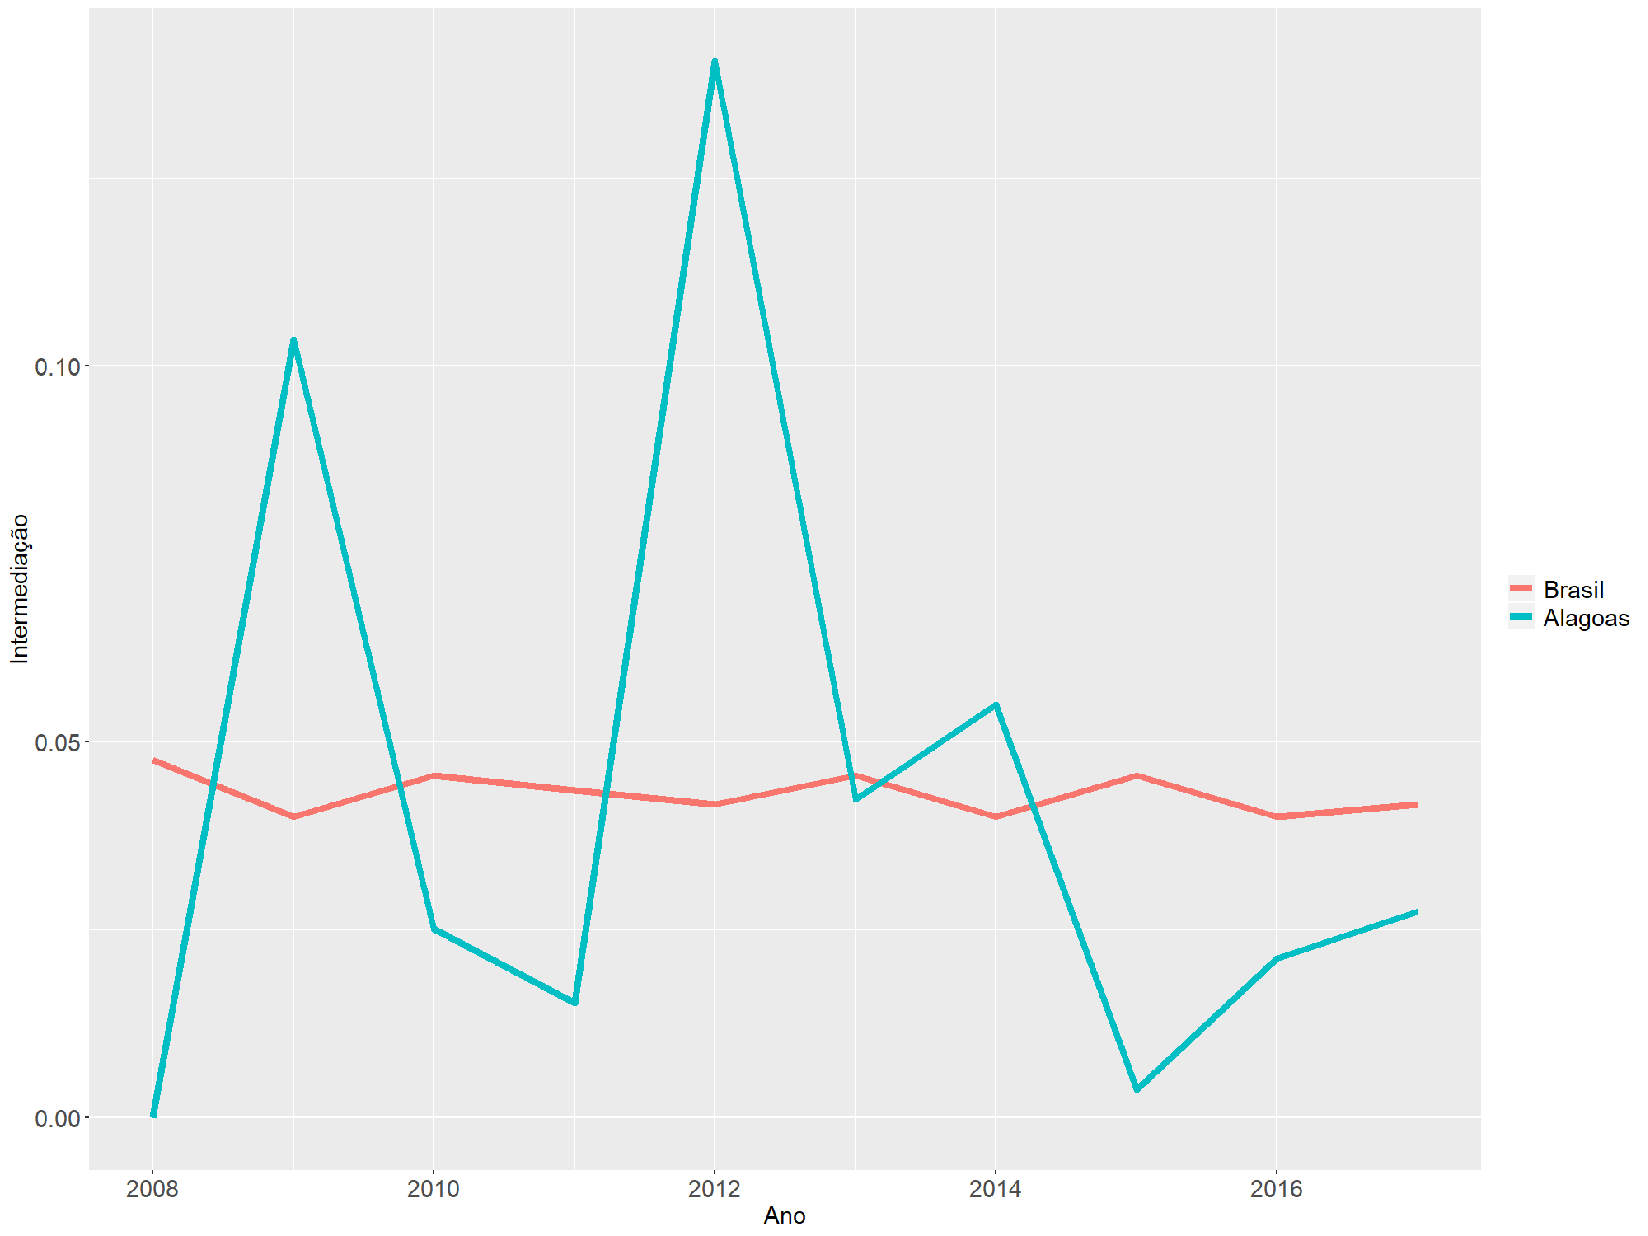
\includegraphics[scale=0.4]{Imagens/exact/graf-linha-betweeness-br-al.pdf}
	\caption{Centralidade de Proximidade (\textit{Exact and Earth Sciences})}
	\label{between-exact-1}
\end{figure}

Na observação dos gráficos da centralidade de intermediação \ref{between-health-1}, \ref{between-agri-1}, \ref{between-exact-1} verificamos que diferentemente do que se observou na centralidade do grau e de proximidade, a relação encontrada entre a Rede Brasil e Alagoas é de uma função matemática não trivial, destacando a sensibilidade dessa medida de centralidade para avaliação da colaboração científica. 


\subsubsection{Health Sciences}

\begin{figure}[H]
	\centering
	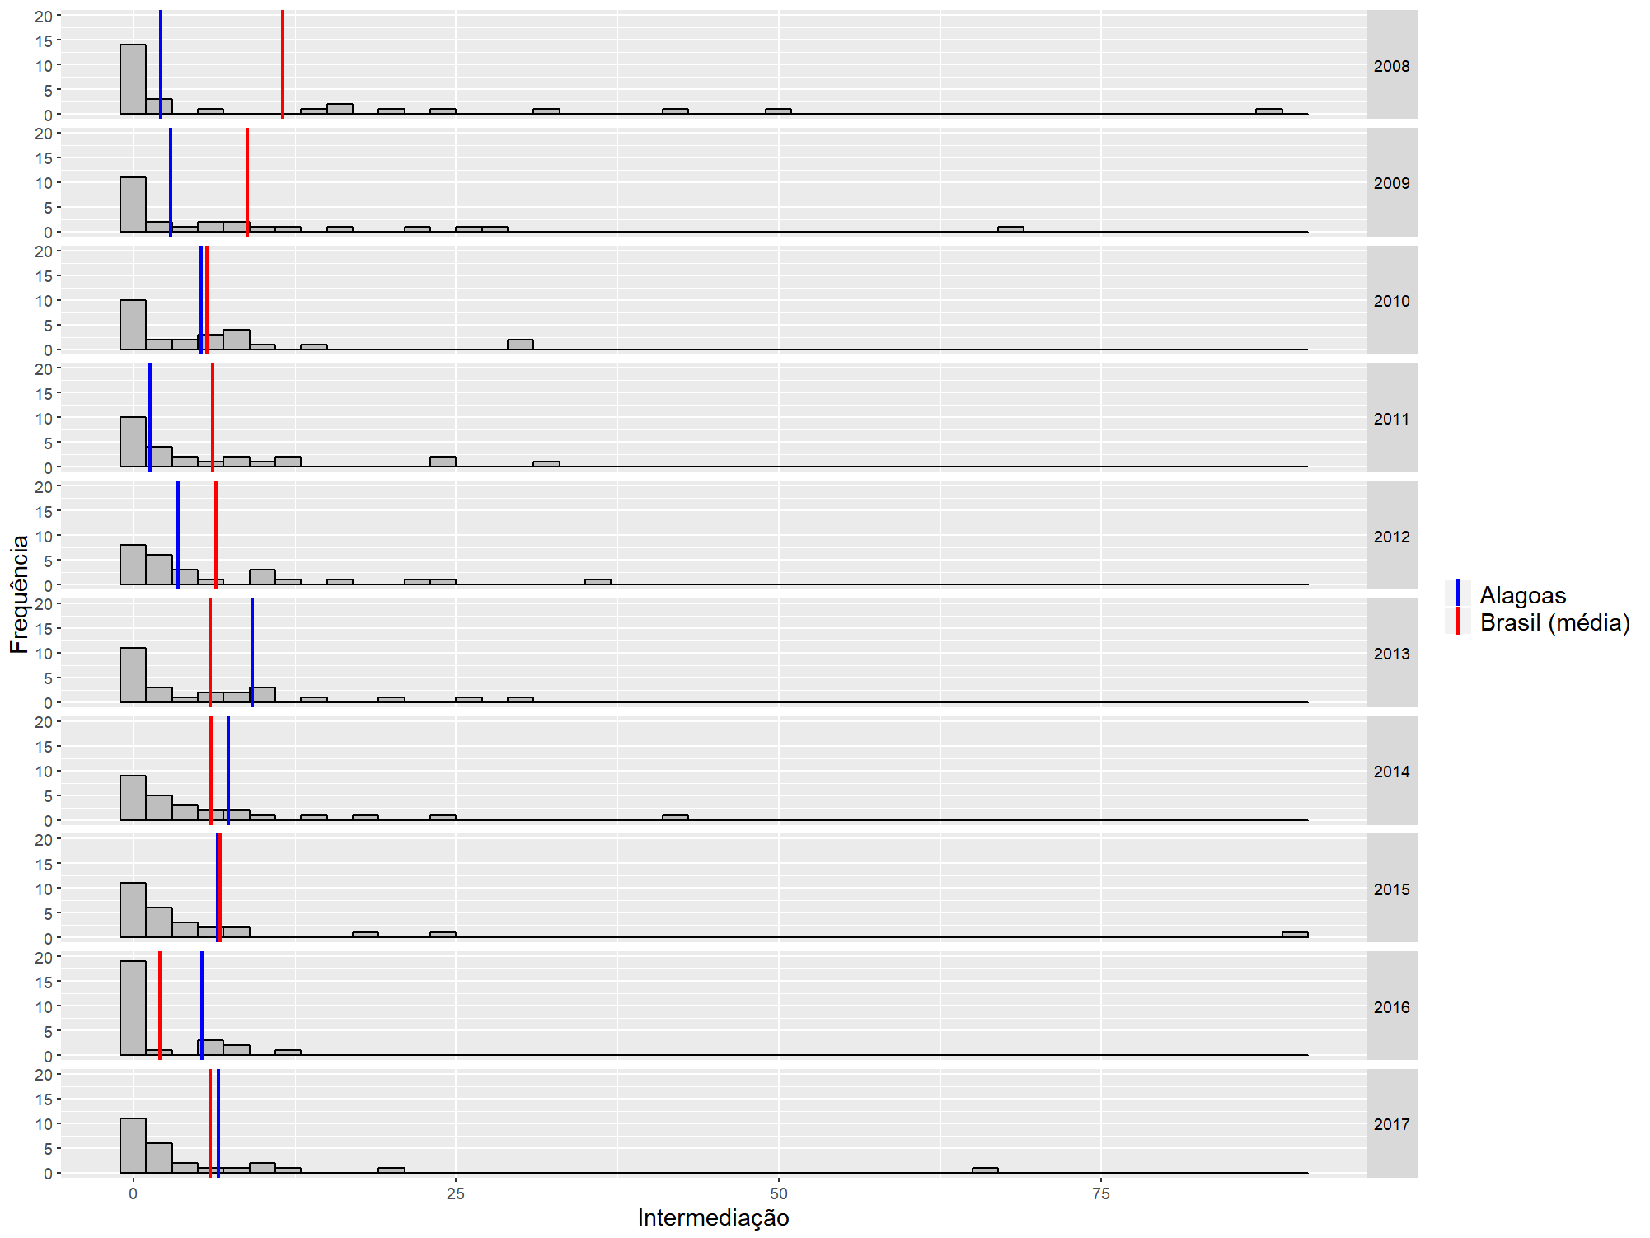
\includegraphics[scale=0.5]{Imagens/betweeness-hist.pdf}
	\caption{Histograma da Centralidade de Proximidade (\textit{Health Sciences})}
       \label{hist-health-between-1}
\end{figure}

\subsubsection{Agricultural Sciences}

\begin{figure}[H]
	\centering
	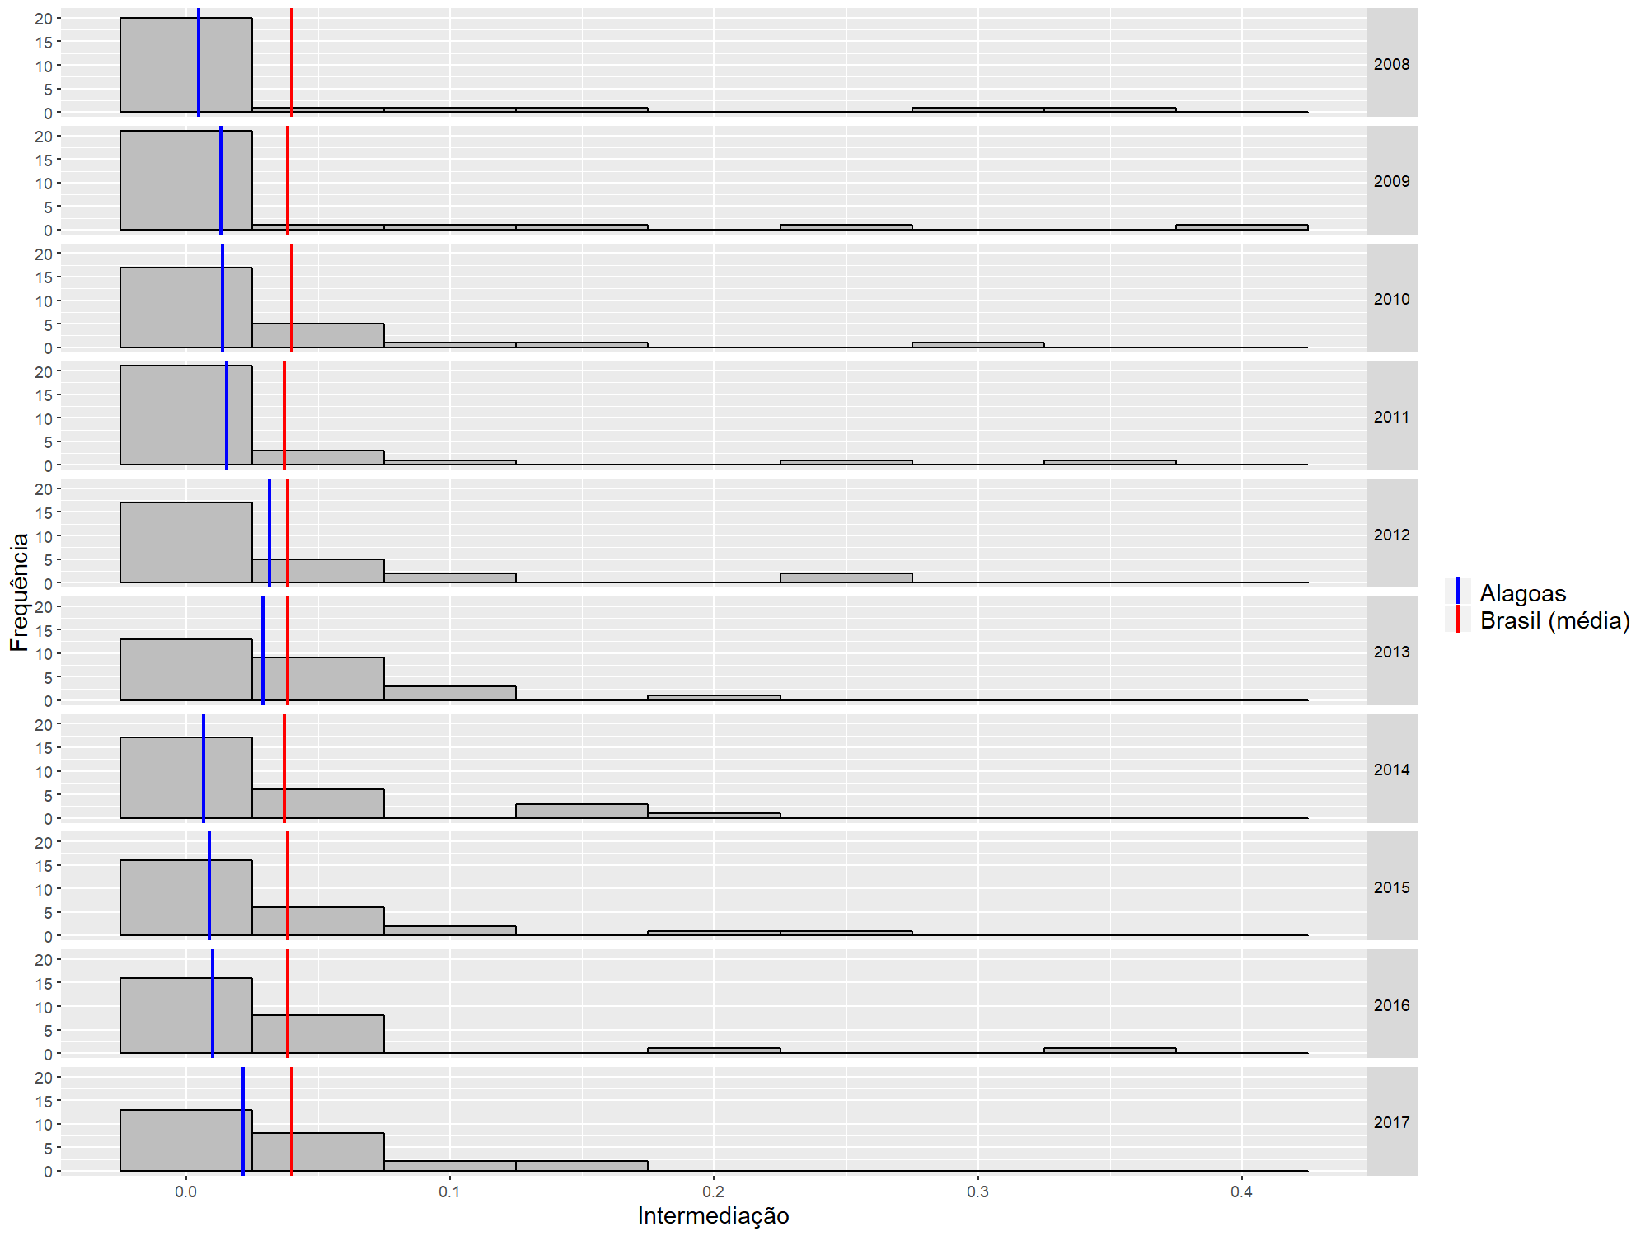
\includegraphics[scale=0.5]{Imagens/agricultural/betweeness-hist.pdf}
	\caption{Histograma da Centralidade de Proximidade (\textit{Agricultural Sciences})}
	\label{hist-agri-between-1}
\end{figure}

\subsubsection{Exact and Earth Sciences}

\begin{figure}[H]
	\centering
	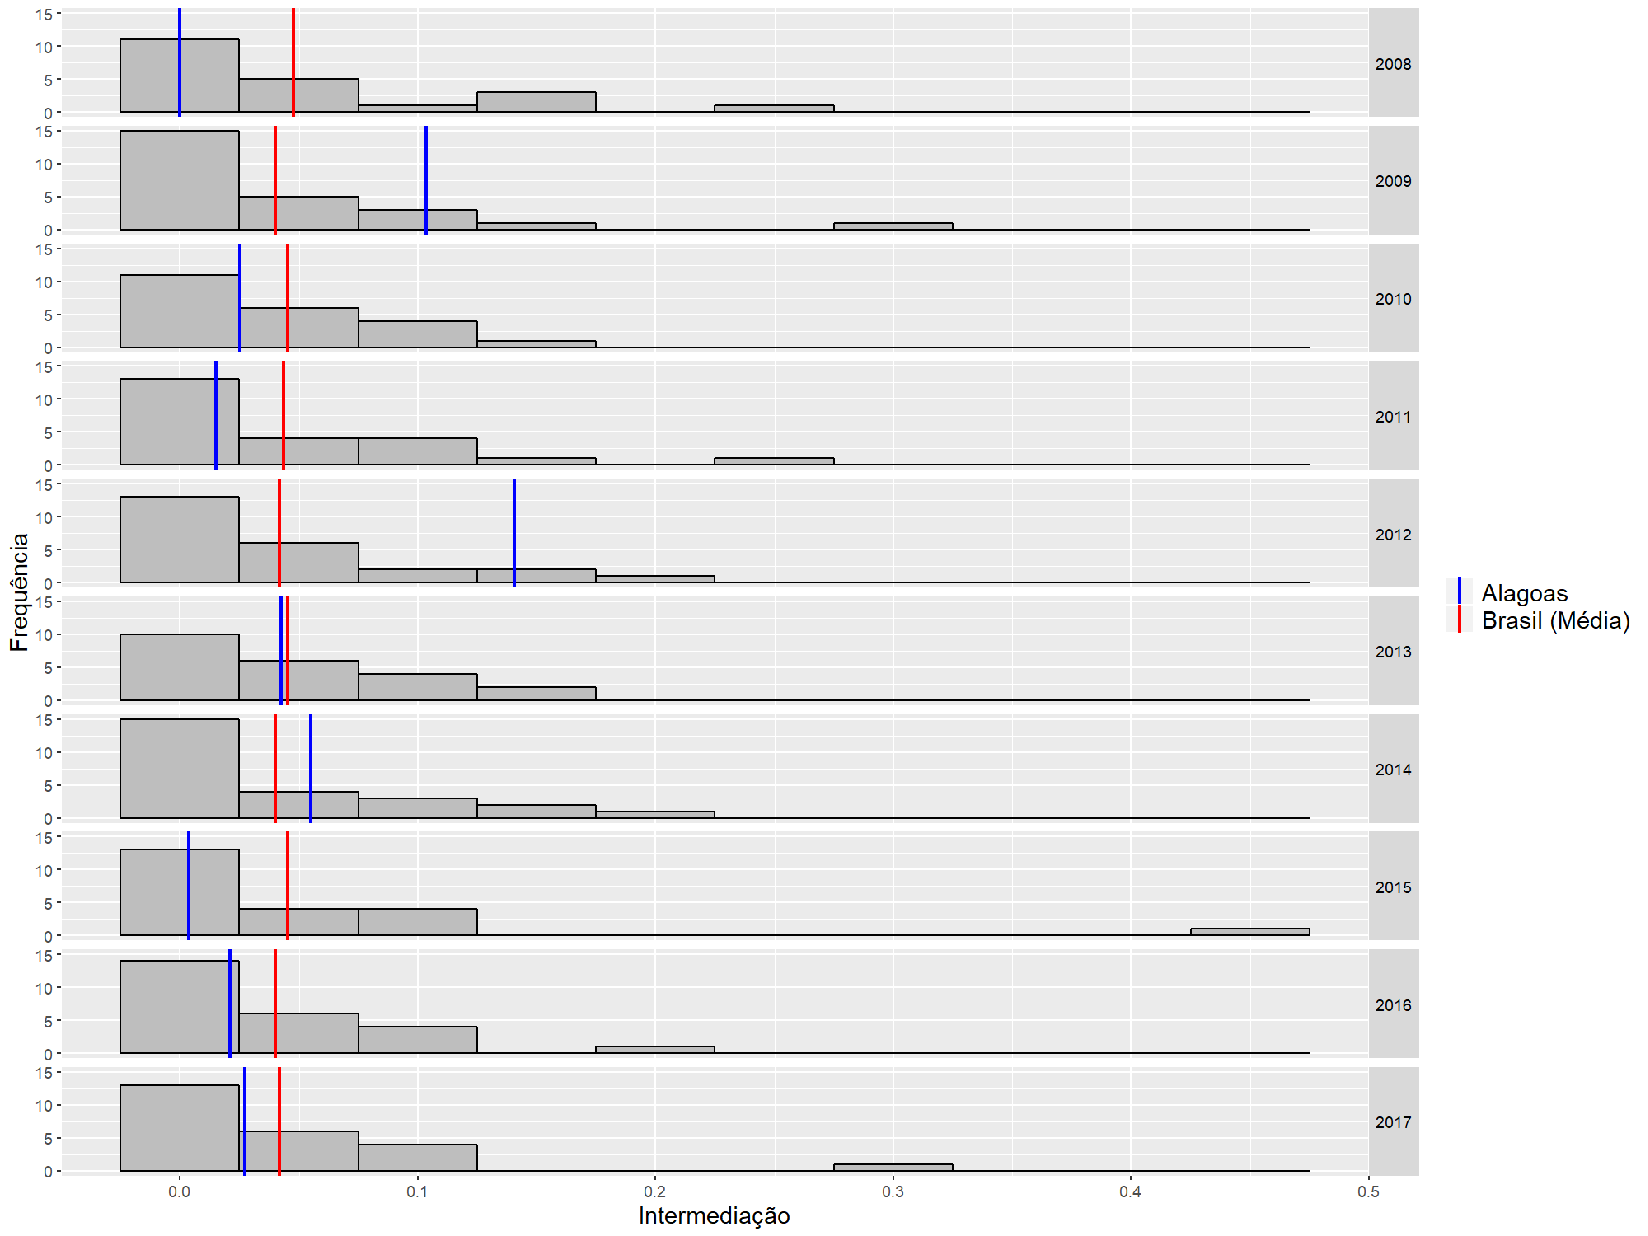
\includegraphics[scale=0.5]{Imagens/exact/betweeness-hist.pdf}
	\caption{Histograma da Centralidade de Proximidade (\textit{Exact and Earth Sciences})}
    \label{hist-exact-between-1}
\end{figure}

%%% TABELA RANKING

\section{\textbf{Ranking das Medidas de Centralidade}}

Nesta seção apresentamos os rankings por Estados (UF) em cada área do conhecimento investigadas neste trabalho. Este ranking tem por objetivo apontar o posicionamento de Alagoas frente a rede Brasil, bem como, por oportuno, mostrar os melhores e piores estados em desempenho para cada medida de centralidade da rede. Os índices foram aferidos pela média da UF em todo o período compreendido entre 2008-2017.

\subsubsection{Ranking: \textit{Health Sciences}}

\begin{table}[H]
	\centering
	\begin{tabular}{|l|l|l|l|l|l|}
		\hline
		\multicolumn{6}{|c|}{\textbf{Ranking das Medidas de Centralidade}}                                                                                                                                                        \\ \hline
		\multicolumn{2}{|c|}{\cellcolor[HTML]{C0C0C0}\textbf{Grau}} & \multicolumn{2}{c|}{\cellcolor[HTML]{C0C0C0}\textbf{Proximidade}}            & \multicolumn{2}{c|}{\cellcolor[HTML]{C0C0C0}\textbf{Intermediação}}          \\ \hline
		UF                          & Média                         & UF                                  & Média                                  & UF                                  & Média                                  \\ \hline
		SP                          & 20,50                         & SP                                  & 0,870                                  & SP                                  & 0,243                                  \\ \hline
		MG                          & 19,60                         & MG                                  & 0,839                                  & MG                                  & 0,145                                  \\ \hline
		RJ                          & 19,00                         & RJ                                  & 0,818                                  & RJ                                  & 0,093                                  \\ \hline
		RS                          & 17,60                         & RS                                  & 0,784                                  & GO                                  & 0,065                                  \\ \hline
		SC                          & 16,90                         & SC                                  & 0,770                                  & CE                                  & 0,060                                  \\ \hline
		PE                          & 16,70                         & PE                                  & 0,765                                  & SC                                  & 0,051                                  \\ \hline
		CE                          & 15,80                         & CE                                  & 0,745                                  & RS                                  & 0,049                                  \\ \hline
		RN                          & 15,20                         & RN                                  & 0,725                                  & PE                                  & 0,038                                  \\ \hline
		BA                          & 14,60                         & \textbf{AL} & \textbf{0,717} & \textbf{AL} & \textbf{0,038} \\ \hline
		\textbf{AL}                 & \textbf{14,50}                & BA                                  & 0,715                                  & RN                                  & 0,032                                  \\ \hline
		PB                          & 14,50                         & PB                                  & 0,707                                  & PR                                  & 0,030                                  \\ \hline
		PR                          & 13,80                         & PR                                  & 0,700                                  & PA                                  & 0,025                                  \\ \hline
		GO                          & 13,40                         & GO                                  & 0,690                                  & AM                                  & 0,023                                  \\ \hline
		ES                          & 12,50                         & ES                                  & 0,678                                  & PB                                  & 0,021                                  \\ \hline
		PA                          & 12,00                         & PA                                  & 0,660                                  & BA                                  & 0,016                                  \\ \hline
		SE                          & 11,40                         & SE                                  & 0,650                                  & RO                                  & 0,016                                  \\ \hline
		MT                          & 10,80                         & AM                                  & 0,641                                  & MA                                  & 0,015                                  \\ \hline
		AM                          & 10,70                         & MT                                  & 0,641                                  & MT                                  & 0,014                                  \\ \hline
		PI                          & 9,90                          & PI                                  & 0,616                                  & ES                                  & 0,012                                  \\ \hline
		MA                          & 9,40                          & MA                                  & 0,614                                  & PI                                  & 0,004                                  \\ \hline
		MS                          & 5,30                          & AP                                  & 0,557                                  & SE                                  & 0,004                                  \\ \hline
		AC                          & 4,90                          & RO                                  & 0,552                                  & AC                                  & 0,001                                  \\ \hline
		RO                          & 4,22                          & MS                                  & 0,538                                  & MS                                  & 0,001                                  \\ \hline
		RR                          & 3,70                          & AC                                  & 0,518                                  & AP                                  & 0,000                                  \\ \hline
		AP                          & 3,63                          & RR                                  & 0,500                                  & DF                                  & 0,000                                  \\ \hline
		TO                          & 2,33                          & TO                                  & 0,495                                  & RR                                  & 0,000                                  \\ \hline
		DF                          & 1,00                          & DF                                  & 0,436                                  & TO                                  & 0,000                                  \\ \hline
	\end{tabular}
	\caption{Ranking Medidas de Centralidade (\textit{Health Sciences})}
	\label{rank-health}
\end{table}

\subsubsection{Ranking: \textit{Agricultural Sciences}}

\begin{table}[H]
	\centering
	\begin{tabular}{|l|l|l|l|l|l|}
		\hline
		\multicolumn{6}{|c|}{\textbf{Ranking das Medidas de Centralidade}}                                                                                                                                    \\ \hline
		\multicolumn{2}{|c|}{\cellcolor[HTML]{C0C0C0}\textbf{Grau}} & \multicolumn{2}{c|}{\cellcolor[HTML]{C0C0C0}\textbf{Proximidade}} & \multicolumn{2}{c|}{\cellcolor[HTML]{C0C0C0}\textbf{Intermediação}} \\ \hline
		UF                          & Média                         & UF                     & Média                                    & UF                              & Média                             \\ \hline
		RN                          & 24,10                         & MG                     & 0,889                                    & MG                              & 0,213                             \\ \hline
		MG                          & 23,20                         & RN                     & 0,877                                    & RN                              & 0,205                             \\ \hline
		PE                          & 17,60                         & RS                     & 0,786                                    & RS                              & 0,115                             \\ \hline
		RS                          & 17,20                         & PE                     & 0,740                                    & PB                              & 0,067                             \\ \hline
		PB                          & 16,60                         & PB                     & 0,718                                    & GO                              & 0,067                             \\ \hline
		RJ                          & 15,80                         & RJ                     & 0,701                                    & PE                              & 0,062                             \\ \hline
		MT                          & 14,40                         & MT                     & 0,675                                    & RJ                              & 0,042                             \\ \hline
		GO                          & 14,10                         & GO                     & 0,665                                    & CE                              & 0,031                             \\ \hline
		CE                          & 13,30                         & CE                     & 0,652            & MT      & 0,031     \\ \hline
		PA                          & 13,30                         & PA                     & 0,651                                    & PA                              & 0,020                             \\ \hline
		PR                          & 12,70                         & BA                     & 0,636                                    & PR                              & 0,020                             \\ \hline
		BA                          & 12,60                         & PR                     & 0,635                                    & MS                              & 0,018                             \\ \hline
		\textbf{AL}                 & \textbf{12,00}                & \textbf{AL}            & \textbf{0,625}                           & PI                              & 0,017                             \\ \hline
		PI                          & 11,80                         & ES                     & 0,625                                    & ES                              & 0,016                             \\ \hline
		ES                          & 11,70                         & PI                     & 0,624                                    & BA                              & 0,016                             \\ \hline
		MS                          & 10,90                         & MS                     & 0,609                                    & \textbf{AL}                     & \textbf{0,015}                    \\ \hline
		SC                          & 9,70                          & TO                     & 0,589                                    & SC                              & 0,009                             \\ \hline
		TO                          & 9,50                          & SP                     & 0,580                                    & SP                              & 0,008                             \\ \hline
		SP                          & 9,20                          & SC                     & 0,576                                    & AC                              & 0,008                             \\ \hline
		SE                          & 8,60                          & SE                     & 0,571                                    & TO                              & 0,008                             \\ \hline
		AM                          & 7,30                          & AC                     & 0,558                                    & AM                              & 0,004                             \\ \hline
		AC                          & 7,00                          & AM                     & 0,544                                    & SE                              & 0,004                             \\ \hline
		MA                          & 7,00                          & RO                     & 0,540                                    & RO                              & 0,003                             \\ \hline
		RO                          & 6,22                          & MA                     & 0,537                                    & MA                              & 0,002                             \\ \hline
		RR                          & 5,50                          & RR                     & 0,526                                    & RR                              & 0,000                             \\ \hline
		DF                          & 2,40                          & AP                     & 0,490                                    & AP                              & 0,000                             \\ \hline
		AP                          & 2,20                          & DF                     & 0,423                                    & DF                              & 0,000                             \\ \hline
	\end{tabular}
	\caption{Ranking Medidas de Centralidade (\textit{Agricultural Sciences})}
	\label{rank-agri}
\end{table}


\subsubsection{Ranking: \textit{Exact and Earth Sciences}}

\begin{table}[H]
	\centering
	\begin{tabular}{|l|l|l|l|l|l|}
		\hline
		\multicolumn{6}{|c|}{\textbf{Ranking das Medidas de Centralidade}}                                                                                                                                             \\ \hline
		\multicolumn{2}{|c|}{\cellcolor[HTML]{C0C0C0}\textbf{Grau}} & \multicolumn{2}{c|}{\cellcolor[HTML]{C0C0C0}\textbf{Proximidade}} & \multicolumn{2}{c|}{\cellcolor[HTML]{C0C0C0}\textbf{Intermediação}}          \\ \hline
		UF                          & Média                         & UF                     & Média                                    & UF                                  & Média                                  \\ \hline
		RJ                          & 13,40                         & MG                     & 0,657                                    & MG                                  & 0,173                                  \\ \hline
		MG                          & 13,30                         & RJ                     & 0,651                                    & RJ                                  & 0,144                                  \\ \hline
		SP                          & 11,40                         & SP                     & 0,618                                    & SP                                  & 0,091                                  \\ \hline
		RS                          & 10,60                         & RS                     & 0,601                                    & RS                                  & 0,071                                  \\ \hline
		PB                          & 9,80                          & RN                     & 0,581                                    & RN                                  & 0,059                                  \\ \hline
		RN                          & 9,70                          & PB                     & 0,566                                    & PE                                  & 0,055                                  \\ \hline
		PE                          & 9,50                          & PE                     & 0,565                                    & PB                                  & 0,054                                  \\ \hline
		PR                          & 9,10                          & BA                     & 0,559                                    & PR                                  & 0,049                                  \\ \hline
		BA                          & 8,70                          & SC                     & 0,556            & \textbf{AL} & \textbf{0,043} \\ \hline
		SC                          & 8,50                          & PR                     & 0,555                                    & CE                                  & 0,043                                  \\ \hline
		CE                          & 8,20                          & CE                     & 0,554                                    & SC                                  & 0,039                                  \\ \hline
		\textbf{AL}                 & \textbf{7,90}                 & \textbf{AL}            & \textbf{0,528}                           & PI                                  & 0,036                                  \\ \hline
		PA                          & 6,20                          & GO                     & 0,512                                    & BA                                  & 0,029                                  \\ \hline
		SE                          & 6,10                          & ES                     & 0,485                                    & GO                                  & 0,029                                  \\ \hline
		GO                          & 6,00                          & SE                     & 0,483                                    & PA                                  & 0,025                                  \\ \hline
		AM                          & 5,60                          & AM                     & 0,480                                    & SE                                  & 0,018                                  \\ \hline
		ES                          & 5,60                          & PA                     & 0,473                                    & MT                                  & 0,013                                  \\ \hline
		PI                          & 5,10                          & PI                     & 0,472                                    & AM                                  & 0,012                                  \\ \hline
		MT                          & 4,67                          & RO                     & 0,442                                    & MA                                  & 0,010                                  \\ \hline
		MS                          & 3,63                          & MT                     & 0,435                                    & ES                                  & 0,006                                  \\ \hline
		MA                          & 3,50                          & MS                     & 0,412                                    & RO                                  & 0,002                                  \\ \hline
		RO                          & 3,25                          & TO                     & 0,411                                    & MS                                  & 0,001                                  \\ \hline
		RR                          & 2,40                          & MA                     & 0,404                                    & AC                                  & 0,000                                  \\ \hline
		TO                          & 2,17                          & RR                     & 0,395                                    & AP                                  & 0,000                                  \\ \hline
		DF                          & 2,00                          & AP                     & 0,388                                    & DF                                  & 0,000                                  \\ \hline
		AP                          & 2,00                          & AC                     & 0,384                                    & RR                                  & 0,000                                  \\ \hline
		AC                          & 1,80                          & DF                     & 0,000                                    & TO                                  & 0,000                                  \\ \hline
	\end{tabular}
	\caption{Ranking Medidas de Centralidade (\textit{Exact and Earth Sciences})}
	\label{rank-exact}
\end{table}


\section{\textbf{Discussão dos Resultados}}

Esta seção tem a por objetivo a discussão dos resultados obtidos neste trabalho, os estudo de redes de coautorias por medidas de centralidade de redes complexas, e a contextualização destes ao comportamento da colaboração científica. A metodologia aplicada permitiu a compreensão das características estruturais das redes, e a determinação destas para os estudos exploratórios.

Utilizando o vértice focal Alagoas, podemos comparar nas três áreas do conhecimento selecionadas para esse trabalho, o estudo das três medidas de centralidade, elencadas por \citet{freeman1991centrality} como essenciais ao estudo de redes.

Numérica e graficamente percebemos que para todas as áreas o comportamento a medida da centralidade de grau e de proximidade para o vértice amostral utilizado e a média parâmetro de estudo, em que estas possuem relações de correlações, quer seja positiva ou negativa, forte ou fraca para cada período (ano) em análise; o que não se observa para a centralidade de intermediação que em todas as áreas apresentou resultados \textit{sui generis} indicando assim, uma sensibilidade desta medida.

%Dentro dos conceitos e propriedades das medidas de centralidade de redes, criamos a seguinte contextualização para a melhor interpretação em redes de coautoria.

%\begin{itemize}
%	\item \textbf{Centralidade do Grau:} \\
%	“Um nó importante está conectado com muitos nós.” \\
%	"Um coautor importante está conectado a muitos coautores.”
	
%	\item \textbf{Centralidade de Proximidade:} \\
%	“Um nó importante faz parte de muitos caminhos". \\
%	"Um coautor importante faz parte de muitos caminhos.” 	
	
%	\item \textbf{Centralidade de Intermediação:} \\
%	“Um nó importante está próximo dos outros nós.” \\
%	"Um coautor importante está próximo dos outros coautores.”
	
%\end{itemize}

As medidas de centralidade utilizadas neste trabalhou permitiu a construção de rankings por área, indicando assim os índices aferidos pelos estados para o período de 2008 a 2017, possibilitando o conhecimento da colaboração científica a partir desses indicadores na base de dados e nas áreas estudadas.

Na área de \textit{Health Sciences} verificamos que conforme o ranking na figura \ref{rank-health} os estados em destaque são: São Paulo, Minas Gerais e Rio de Janeiro são os estados que possuem os maiores índices das medidas de centralidade: de grau, de proximidade, de intermediação. Alagoas assume a décima posição junto com Pernambuco para a centralidade do grau. E a nona posição para centralidade de proximidade e de intermediação, nesta última em empate também com Pernambuco.

Em \textit{Agricultural Sciences} o destaque é para os estados do Rio Grande do Norte, Minas Gerais e Rio Grande do Sul (conforme ranking \ref{rank-agri}); tendo Alagoas assumido respectivamente as posições de décimo terceiro para centralidade do grau e de proximidade; décimo sexto para intermediação. 

Salientamos que outros estudos exploratórios podem realizar detalhamentos a respeito de comunidades e cliques existentes na rede, a fim de encontrar padrões de relacionamentos interinstitucionais. 

Neste trabalho, a análise proposta traz à tona um conhecimento até então desconhecido, a avaliação da colaboração científica pelas redes de coautoria no período de 2008 a 2017, base SciELO das áreas estudadas. E que as medidas com suas respectivas propriedades podem subsidiar estudos investigativos e exploratórios para a avaliação de outras redes, e fatores que possam influenciar o comportamento delas.
